\documentclass[]{article}
\usepackage[UTF8]{ctex}
\usepackage{amsmath}
\usepackage{graphicx}
\usepackage{ulem}
\newtheorem{theorem}{Theorem}
\newtheorem {definition}{Definition}
\usepackage{tikz}
\usepackage{float}

%opening
\title{保密系统的通信原理\footnote{原始论文信息: Shannon C E . Communication Theory of Secrecy Systems[J]. Bell System Technical Journal, 1949, 28(4):656–715.}}
\author{C. E. Shannon\\
{\small  翻译:李晓峰,北京联合大学智慧城市学院\footnote{译者email:cy\_lxf@163.com,译文来自于译者发起的“信息安全经典翻译”开源项目https://gitee.com/uisu/InfSecClaT}}
}

\usepackage{hyperref} %生产书签

\begin{document}
	
\maketitle
	
\newpage
\tableofcontents
\newpage

%---------------------------------------------
%   
%     1.INTRODUCTION AND SUMMARY
%
%---------------------------------------------
	
	\section{引言和概述(INTRODUCTION AND SUMMARY)}
	密码学和保密系统问题是通信理论的一个有意思的应用\footnote{Shannon, C. E., “ A Mathematical Theory of Communication , ”
	Bell System Technical Journal, July 1948 , p. 379 ; Oct. 1948 , p.623 .}。本文提出了一种保密系统理论,该方法在理论层面上,旨在补充密码学研究方法\footnote{See , for example , H . F . Gaines , “ Elementary Cryptanalysis , ” or M . Giviergc ,“ Cours de Cryptographic .”}。在以前工作里,对许多标准类型的编码和密码以及破解它们的方法进行了详细的研究。本文将更加关注保密系统的一般数学结构和性质。\par


本文处理方法在某些方面受到限制。首先,一般有三种类型的保密系统:\\
(1)隐蔽系统,包括隐形墨水、在文本中隐藏消息、或密码隐藏在假消息中,其他对敌人隐藏消息的方法;\\
(2)隐私系统,例如语音反转,其中需要特殊设备来恢复信息;\\
(3)“真实”保密系统,其中信息的含义被密码、
编码等隐藏,虽然它的存在并不隐蔽,而且假定敌人拥有拦截和记录传输信号所需的任何特殊设备。\\
我们认为只有第三种类型的保密系统是心理上可以接受的技术型的保密系统。
\par

其次,文章讨论仅限于离散信息的情况,其中要加密的消息由一系列离散符号组成,每个符号从有限的集合中选择。这些符号可以是一种语言中的字母、一种语言中的单词、“量化”语音或视频信号的振幅等,但是主要关注与字母有关的情况。
\par

本文分为三个部分。现在将简要总结论文主要结论。第一部分论述保密系统的基本数学结构。正如在通信理论中一样,一种语言被看做一个随机过程,这个随机过程根据某个概率系统产生一个离散的符号序列。与语言相关联的是一个特定的参数D,我们称之为语言的冗余。从某种意义上说,D衡量的是语言中的文本在不丢失任何信息的情况下可以缩短多少长度。举个简单的例子,因为在英语单词中u总是跟在q后面,所以u可以省略而不会丢失含义。由于语言的统计结构、某些字母或单词的高频次等原因,英语中可能会有相当多的冗余,冗余在保密系统的研究中至关重要。\footnote{译者注:如果我们把任何字母看成是一个二进制流,那么这种冗余是否就不存在了呢?答案是:一定存在,只不过其表现形式变为重复的二进制块等形式。}
\par

保密系统被抽象地定义为一个空间(可能的消息集)到第二个空间(可能的密文集)的一组变换。集合的每个特定变换对应于使用特定密钥进行加密。这些变换被认为是可逆的(非奇异的)\footnote{译者注:奇异函数(singularity function)是指函数本身有不连续点,也称为脉冲函数,在信号分析中经常用到。非奇异变换是指这个编号完全可逆。},因此当密钥已知时,可以进行唯一的解密。\par

在每个变换下,每个密钥都有一个与变换相关的先验概率,也就是选择此密钥的概率。类似地,假设每个可能的消息都有一个相关的先验概率,由底层的随机过程决定。这些不同密钥和消息的概率实际上是敌方密码分析员对相关选择的先验概率,代表了他的先验知识。\par

要使用保密系统,首先选择一个密钥并将其发送到接收点。密钥的选择确定了系统的特定变换。然后选择一条消息,并将与所选密钥对应的特定变换应用于该消息,以生成密文。该密文通过信道传输到接收点,并可能被“敌人”\footnote{“敌人”一词源于军事应用,在密码工作中常用来表示任何可能拦截密码的人。}截获,在接收端,将特定变换的逆运算应用于密文,以恢复原始消息。\par

如果敌人截获了密文(cryptogram),他可以从中计算出可能产生该密文的各种可能消息和密钥的后验概率。这组后验概率构成了他在拦截后对密钥和消息的知识。因此,“知识”被认为是一组与概率相关的命题。后验概率的计算是密码分析的一般性问题。
\par

作为这些概念的一个例子,在带有随机密钥的简单替换密码中有26!种变换\footnote{译者注:我们可以把26个字母看成26个盒子,从A~Z依次排好,盒子外面写上字母,盒子里面放变换后的字母,那么我们可以很容易计算共有26!中放法。},
对应于26!方式,我们可以选择一种来替换26个不同的字母。每种选择的可能性是一样的,因此每个都有一个先验概率$1/26!$。如果这应用于“普通英语”,密码分析员被假定除了知道是英语文本之外对消息源一无所知,那么N个字母的各种消息的先验概率仅仅是它们在普通英语文本中的相对出现频度。\par

如果敌人在这个系统中截获N个密文字母,他的概率就会改变。如果N足够大(比如50个字母),通常会有一条后验概率几乎为1的消息,而所有其他消息的总概率几乎为零。因此,密文有唯一“解”。对于较小的N(假设N=15),通常会有许多概率相当的消息和密钥,没有一个接近1。在这种情况下,密文有多个“解”。\par

考虑到一个保密系统可表示为一组元素到另一组元素的一组转换,自然存在两种组合操作,可以从给定的两个系统生成第三个系统。第一组合操作被称为乘积操作,对应于用第一保密系统R对消息进行加密,并用第二系统S对所得密文进行加密,R和S的密钥被独立选择。这个整体操作是一个保密系统,其变换由S变换与R变换的乘积组成。概率是两个变换的概率的乘积。\par

第二种组合操作是“加权加”。\[T=pR+qS \ \ \ \  p+q=1\]

这相当于对系统R或S分别以概率p和q做出初步选择\footnote{译者注:这种表达方式怎么表达选择R的概率为p,选择S的概率为q?我觉得这是一种形式化的表达方式,并不是T的某个值,是R和S的加权平均,只是一个形式化的写法。},当这样做时,R或S按照最初定义使用。


研究表明,具有这两种组合运算的保密系统本质上形成了具有单位元素的“线性结合代数”,这是数学家广泛研究的代数变体。


在许多可能的保密系统中,有一种类型具有许多特殊属性。这种类型我们称之为“纯”系统。我们称一个系统是纯的,如果所有密钥的可能性相等,并且如果集合中的任何三种变换$T_i,T_j,T_k$,它们乘积	
\[T_iT^{-1}_jT_k\]
也是这个集合上的变换,也就是说,使用任意三个密钥进行加密、解密和加密必须等同于使用某个密钥进行的加密。
	
对于纯密码,所有密钥本质上是等价的,它们都导致相同的后验概率集,此外,当一个密文被截获时,有一组消息对应这个密文(剩余类)\footnote{译者注:这组消息就是可能产生此密文的所有消息组成。},并且这个类中消息的后验概率与先验概率成比例。敌人截获密码获得的所有信息都是剩余类的具体描述。许多常见密码都是纯系统,包括使用随机密钥的简单替换。在这种情况下,剩余类由与截获密文相同的字母重复模式的所有消息组成。

如果存在一个变换$A$,其逆变换存在且为$A^{-1}$,则两个系统R和S“相似”,当且仅当:
\[R=AS.\]

如果R和S相似,加密结果之间可以建立一对一的对应关系,导致相同的后验概率。两个系统在密码分析上是相同的。


论文的第二部分讨论了“理论保密”(“ theoretical secrecy” )问题。当敌人有无限的时间和人力来分析截获的密码时,系统面对密码分析的安全性如何?该问题与存在噪声的通信问题密切相关,为通信问题而提出的熵(entropy)和疑义度(equivocation)可直接应用于密码学。


“完全保密”(“ Perfect Secrecy ” )的定义是要求系统在密码被敌人截获后,各种消息的密文后验概率与截获前相同消息的先验概率相同。这表明完全保密是可能的,但如果消息数量有限,需要有相同数量的可能密钥。如果消息被认为是以给定的“速率”R(稍后定义)不断生成的,则密钥必须以相同或更高的速率生成。


如果使用具有有限密钥的保密系统,并且截获了N个密文字母,那么对于敌人来说,该密文以一定概率对应一组消息。随着N的增加,域通常会缩小,直到最终有一个唯一的密文“解”,这意味着一个消息的概率基本为1,而所有其他消息概率接近0。定义了一个量$H(N)$,称为“疑义度”(equivocation,原意为“含糊其辞”),它以统计方式测量N个字母密文与唯一解的平均接近程度;也就是说,在截获一个由N个字母组成的密文后,敌人对原始消息的不确定性有多大。推导出了“疑义度”的各种性质,例如,密钥的“疑义度”永远不会随着N的增加而增加,这种“疑义度”是一种理论上的保密指数,理论上,它允许敌人有无限时间分析密码。


确定了称为随机密码的这种理想化类型密码的函数$H(N)$,经过某些调整,该函数可应用于许多实际情况。这提供了一种计算获得保密系统解决方案所需截获材料数量的近似方法。从分析中可以看出,对于普通语言和常用密码类型(不是编码)这个“唯一解距离”大约是$H(K)/D$。这里,$H(K)$是一个测量密钥空间“大小”的数字。如果所有密钥都是先验的,那么$H(K)$是可能的密钥数的对数。D是语言的冗余度,并度量此语言上的“统计约束”。对于随机密钥简单替换,$H(K)$是$log_{10}26!$或大约20,而D(每个字母的十进制数字)在英语中约为0.7。因此,在大约30个字母处出现唯一解。


有可能为“某语言”构造具有有限密钥的保密系统,当$N\rightarrow \infty$时,其不确定性不接近零。在这种情况下,无论截获了多少材料,敌人仍然无法获得密码的唯一解,仍有许多有合理概率的选择,这种系统我们称之为理想系统。在任何语言中都有可能近似这种行为,换言之,可以后退到任意大的$N$使$H(N)$接近零。然而,这种系统有许多缺点,例如密码传输的复杂性和对错误的敏感性。

论文的第三部分涉及“实际保密”(“practical secrecy”)。当截获$N$个字母时,具有相同密钥大小的两个系统可能都是唯一可解的,但在实现该解决方案所需的劳动量上存在很大差异。分析了保密系统的基本弱点。这产生了构建需要大量工作才能解决的系统的方法。最后,讨论了保密系统各种期望之间的某种不兼容性。

\newpage

\begin{center}
	\section*{第一部分\ 保密系统的数学结构(MATHEMATICAL STRUCTURE OF SECRECY SYSTEMS)}
\end{center}

%---------------------------------------------
%   
%     2.SECRECY SYSTEMS
%
%---------------------------------------------

\section{保密系统(SECRECY SYSTEMS)}

作为密码学数学分析的第一步,以数学上可接受的方式定义我们所说的保密系统。图\ref{Fig:fig1}中显示了一般保密系统的“示意图”。在发送端有两个信息源:消息源和密钥源。密钥源从系统中可能的密钥中产生特定密钥。该密钥通过某种方式发送,消息源产生一条消息(“明文”),该消息被加密,将生成的密文发送给接收端,敌手通过可能的可拦截手段(例如无线电)。在接收端,密文和密钥在解密器中组合以恢复消息。
\par

\begin{figure}[htbp]
	\centering
	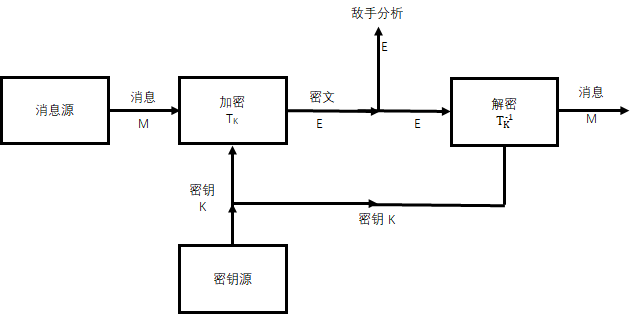
\includegraphics[width=0.8\textwidth]{general-secrecy-system.png}
	\caption{一般保密系统示意图}
	\label{Fig:fig1}
\end{figure}

显然,加密程序执行函数操作。如果$M$是消息,$K$是密钥,$E$是加密消息或密文,我们有\[E=f(M,K)\],即$E$是$M$和$K$的函数。然而,最好不要将其视为两个变量的函数,而是视为(一个参数)操作或变换族,写为\[E=T_iM.\]
变换$T_i$应用于消息$M$产生密文$E$。索引$i$对应于所使用的特定密钥。

通常,我们假设只有有限数量的可能密钥,并且每个密钥都具有概率$p_i$。因此,密钥源由统计过程或装置表示,该统计过程或装置从具有相应概率$p_1,p_2\cdots,p_m$的变换集合$T_1,T_2,\cdots,T_m$中选择一个,同样,我们假定有一个有限多个可能的消息$M_1,M_2,\cdots,M_n$,可能的消息对应的先验概率为$q_1,q_2,\cdots,q_n$,可能消息是正常长度为$N$的英文字母序列,相关概率是这些序列在正常英文文本中出现的相对频率。

在接收端,必须能够恢复$M$,知道$E$和$K$。因此,族中的变换$T_i$必须具有唯一的逆$T^{-1}_i$,使得$T_iT^{-1}_i=I$,$I$即恒等式变换,我们有:\[M=T^{-1}_i E.\]

无论如何,该逆必须对每个$E$唯一存在,E可以由密钥$i$和M确定。因此,我们得出了这样的定义:\textbf{保密系统是一组可能消息到一组密文的唯一可逆变换$T_i$的族,该变换$T_i$具有相关联的概率$p_i$。这种类型系统都称为“保密系统”。}为了方便起见,可能的消息集称为“消息空间”,可能的密文(cryptgrams)集称为"密文空间"。

如果两个保密系统由相同的变换集$T_i$组成,具有相同的消息和密文空间(范围和域)以及相同的密钥概率,则它们将是相同的。\footnote{译者注:这里其实是定义了“保密系统”的相等关系。}

保密系统可以被机械地视为一台机器,上面有一个或多个控件。一个字母序列,即消息,被输入到机器的输入端,第二个序列出现在输出端。控件的特定设置对应于使用的特定密钥。必须确定某种统计方法,从所有可能的密钥中选择密钥。

为了使问题在数学上易于处理,我们假设敌人知道正在使用的系统。也就是说,他知道变换族$T_i$和选择各种密钥的概率。可能会有人反对这种假设是不现实的,因为密码分析员通常不知道使用了什么系统,也不知道概率。对于这个反对意见有两个答案:

1.由于我们对保密系统的宽泛定义,这种限制比最初看起来要弱得多。假设密码学者截获了一条消息,并且不知道是否使用了替换、换位或维吉尼亚型(Vigen\`{e}re)密码。 他可以认为消息是由一个系统加密的,其中密钥一部分表示使用哪种类型,密钥剩下一部分是该类型的特定密钥。这三种不同的可能性被分配概率,依据相应类型密码的加密者的先验概率的最佳估计。


2. 这一假设实际上是密码研究中通常使用的假设。它是悲观的,因此是安全的,但从长远来看是现实的,因为人们必须明白自己的系统最终会被破解。因此,即使设计了一个全新的系统,在其没被发现的情况下,敌人无法为其分配任何先验概率,一个人仍然必须对自己最终获得相关知识抱有期望。(Thus even when an entirely new system is devised , so that the enemy cannot assign any a priori probability to it without discovering it himself , one must still live with the expectation of his eventual knowledge .)

这种情况类似于游戏\footnote{ See von Neumann and Morgenstern	"The Theory of Games" Princeton 1947}理论中的情况,假设对手“发现”正在使用的游戏策略。这两种情况下,假设都用来清晰地描绘对手的知识。


对我们的保密系统定义的第二个可能的反对意见是,没有考虑到在消息中插入空值和使用多个替代项的常见做法。在这种情况下,给定消息和密钥没有唯一的密文,但加密者可以随意从许多不同的密文中选择。这种情况可以处理,但在现阶段只会增加复杂性,而不会实质上改变任何基本结果。

如果消息是由"通信的数学原理"一文中所述类型的Markoff过程生成的,以此表示信息源,则各种消息的概率由Markoff过程的结构决定。然而,目前,我们希望更全面地了解情况,并将消息仅视为具有相关概率的抽象实体集,不一定由字母序列组成,也不一定由Markoff过程产生。

需要强调的是,在本文中,保密系统不是指一个,而是指一组多个变换。在选择密钥后,只使用其中一个变换,并由此将保密系统定义为语言上的单个变换。然而,敌人不知道选择了什么密钥,“可能”的密钥对他来说与实际的密钥一样重要。\textbf{事实上,只有这些其他可能性的存在才使系统具有保密性}。由于保密性是我们的基本关心点,我们需要使用上文定义的详细的保密系统概念。这种情况中可能性和现实一样重要,在游戏策略中经常发生。国际象棋游戏的过程很大程度上受到威胁的控制,而这些威胁并未实施。在某种程度上类似于游戏理论中未实现假设的“虚拟存在”。

可以注意到,在我们的定义下,语言上的单个操作形成了一种退化类型的保密系统————一个只有一个单位概率密钥的系统。这样的系统没有保密性————密码分析员通过应用该变换的逆来发现消息,该变换是系统中唯一的一个,在这种情况下,解密者和密码分析员拥有相同的信息。一般来说,解密者的知识和敌方密码分析者的知识之间的唯一区别是解密者知道正在使用的特定密钥,而密码分析员只知道集合中各种密钥的先验概率。解密的过程是将加密中使用的特定变换的逆应用于密码。密码分析的过程是在只给出密文和各种密钥和信息的先验概率下,试图确定消息(或特定密钥)。

当应用于实际情况时,有许多与保密理论有关的困难的认识论问题(difficult epistemological questions),事实上,与任何涉及概率问题(特别是先验概率、贝叶斯定理等)并应用于物理情境的理论都存在这些难题。从抽象的角度来看,概率论可以通过测度理论方法建立在严格的逻辑基础上。\footnote{See J . L . Doob , “ Probability as Measure , ” Annals of Math . Statv . 12 , 1941 , pp .206 - 214 .} \footnote{A . Kolmogoroff ,“ Grundbegriffe der Wahrscheinlichkeits rechnung , ” Ergebnisse der Mathematic , v . 2 , No . 3 ( Berlin 1933 ) .}
然而,当应用于实际情况时,尤其是当涉及“主观”概率和不可重复实验时,存在许多逻辑有效性问题。例如,在这里提出的保密方法中,假定敌方密码学家已知各种密钥和消息的先验概率————如何根据他对情况的了解基础上,确定他估计值是否可操作?

我们可以构建“瓮与死”( urn and die)类型的人工密码,其中先验概率具有明确含义,这里使用的理想化当然是合适的。在其他情况下,我们可以想象,例如,火星入侵者之间的拦截通信,先验概率可能非常不确定,以至于没有意义。大多数实际的密码情况介于这些限制之间。密码分析师可能愿意将可能的消息分类为“合理”、“可能但不像”和“不合理”,但觉得更精细的细分没有意义。

幸运的是,在实际情况下,只有密钥和消息的先验概率中出现极端错误时,才会导致重要参数产生显著误差。这是因为消息和密文数量呈指数行为,以及采用的对数度量。

\newpage

%---------------------------------------------
%   
%     3.REPRESENTATION OP SYSTEMS
%
%---------------------------------------------

\section{系统的表示(REPRESENTATION OP SYSTEMS)}
如上定义的保密系统可以以各种方式表示。如图\ref{Fig:fig2}和图\ref{Fig:fig4}所示,使用线图表示。可能的消息由左边的点表示,可能的密文由右边的点表示。如果某个密钥,如密钥1,将消息M2转换为密文E4,则M2和E4由标记为1的线连接,以此类推。从每一条可能的消息中,每一个不同的密钥都必须出现一行。如果每一个密文都是这样,我们将说系统是\textbf{封闭}的。

\begin{figure}[htbp]
	\centering
	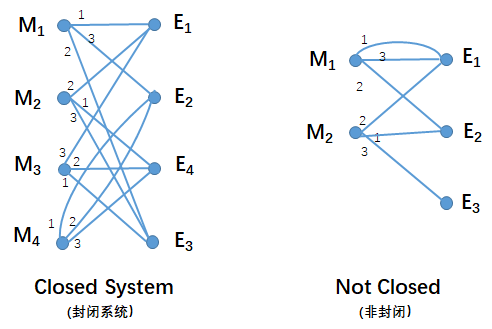
\includegraphics[width=0.8\textwidth]{fig-2.png}
	\caption[简单系统的线条图]{简单系统的线条图\footnote{译者注:原文左边图没有$E_1,E_2,E_3,E_4$的标注,根据文中内容加上了。}}
	\label{Fig:fig2}
\end{figure}

描述系统的一种更常见的方法是说明如何利用密钥对消息进行运算获得密文。类似地,我们通过如何选择密钥定义各种密钥的概率,或根据敌人选择密钥的习惯来定义。消息的概率是由先验知识来隐式确定的,这些知识包括敌人语言习惯,战术情况(这将影响消息的可能内容)以及我们可能拥有的关于密文的任何特殊信息。

\newpage

%---------------------------------------------
%   
%     4.SOME EXAMPLES OF SECRECY SYSTEMS
%
%---------------------------------------------

\section{保密系统的一些例子(SOME EXAMPLES OF SECRECY SYSTEMS)}

在本节中,将给出一些密码的示例。为了便于说明,这些示例在本文的其余部分经常引用。

\subsection{简单替换密码(Simple Substitution Cipher )}
在这种密码中,消息中的每个字母都被一个固定的替代字母代替,通常也是一个字母。消息:
\[M=m_1 m_2 m_3 m_4\cdots\]
此处$m_1,m_2,\cdots$是连续的字母,变成:
\begin{equation}
\begin{aligned}
	E &=e_1 e_2 e_3 e_4 \cdots \\
	&= f(m_1)f(m_2)f(m_3)f(m_4)\cdots\nonumber
\end{aligned}
\end{equation}
此处$f(m)$函数有逆函数,密钥是字母表的排列(当替代物是字母时),例如$X G U A C D T B F H R S L M Q V Y Z W I E J O K N P$,在这个例子中,第一个字母$X$是$A$的替代物,$G$是$B$的替代物等。


\subsection{换位(固定周期d)(Transposition (Fixed Period d))}
消息被分为长度为$d$的组,有一个置换作用于第一组,相同置换作用于第二组,以此类推。置换是密钥,可以由前$d$个整数的置换表示。因此,对于d=5,我们可能有2 3 1 5 4作为置换。这意味着:
\begin{equation}
	\begin{aligned}
		&m_1\ m_2\ m_3\ m_4\ m_5\textbrokenbar \ m_6\ m_7 \ m_8 \ m_9 \ m_{10}\textbrokenbar \cdots\text{变换为} \\
		&m_2\ m_3\ m_1\ m_5\ m_4\textbrokenbar \ m_7\ m_8 \ m_6 \ m_{10} \ m_9\textbrokenbar \cdots\nonumber
	\end{aligned}
\end{equation}
两个或多个换位依次应用被称为复合换位(compound transposition)。如果周期为$d_1,\cdots,d_s$,很明显,结果是周期$d$的换位,其中$d$是$d_1,\cdots,d_s$的最小公倍数。

\vspace{1cm}
***********************************************************\par
\textsl{\textbf{译者注:我们用下面一张图来解释加密过程:}}\par
	\begin{figure}[htb]
		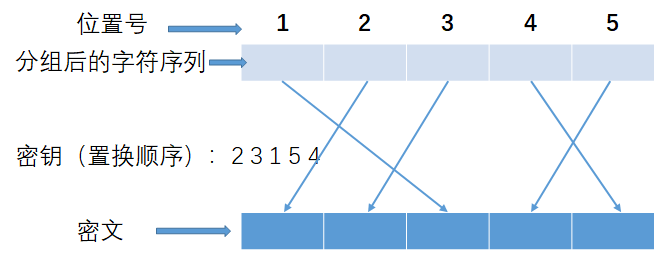
\includegraphics[width=0.8\textwidth]{transpostion-fixedp.png}
	\end{figure}
\par
***********************************************************\par
\vspace{1cm}

\subsection{维吉尼亚及其变种(Vigen\`{e}re and Variations )}
在维吉尼亚密码中,密钥由$d$个字母序列组成。这些字母在消息下方重复书写\footnote{译者注:看下面的图,看着图比较容易理解此话。},消息和密文模26加(考虑字母表编号从$A=0到Z=25$),即
\[ e_i = m_i+k_i(mod\ 26) \]
此处$k_i$是周期$d$中第$i$个元素,例如,密钥为$G\ A\ H$,我们可以得到:
\begin{equation}
	\begin{aligned}
	message\ &N\ O\ W\ I\ S\ T\ H\ E\ &\cdots\\
	repeated\ key\ &\underline{G\ A\ H}\ \underline{G\ A\ H}\ \underline{G\ A\ H}\ G\ A\ &\cdots\\
	cryptgram\ &T\ O\ D\ O\ S\ A\ N\ E\ &\cdots\nonumber
	\end{aligned}
\end{equation}

\vspace{1cm}
***********************************************************\par
\textsl{\textbf{译者注:}}\par
上面的计算过程,我们解释一下,首先我们要获得字母对应的数字:\par
\begin{tabular}{|c|c|c|c|c|c|}
	\hline 
	A=0& B=1 & C=2 & D=3 & E=4 & F=5 \\ 
	\hline 
	G=6& H=7 & I=8 & J=9 & K=10 & L=11 \\ 
	\hline 
	M=12& N=13 & O=14 & P=15 & Q=16 & R=17 \\ 
	\hline 
	S=18& T=19 & U=20 & V=21 & W=22 & X=23 \\ 
	\hline 
	Y=24& Z=25 &  &  &  &  \\ 
	\hline 
\end{tabular} 
\par
那么上面的方程就可以写成\par
\begin{equation}
\begin{aligned}
message\ &13\ &14\    &22\ &8\ &18\ &19\ &7\ &4\ &\cdots\\
repeated\ key\ &6\ &0\ &7\ &6\ &0\ &7\   &6\ &0\ &\cdots\\
cryptgram\ &19\ &14\   &3\ &14\ &18\ &0\ &13\ &4\ &\cdots\nonumber
\end{aligned}
\end{equation}

\par
***********************************************************\par

周期1的Vigen\`{e}re被称为凯撒密码\footnote{译者注:很多资料中称凯撒密码为加3模26的运算,此处显然是将凯撒密码扩展为加法密码。}。它是一种简单的替换,其中$M$的每个字母在字母表中前进一个固定的量。这个量是密钥,可以是从0到25的任何数字。所谓的波弗特(Beaufort)和变异波弗特(Variant Beaufort)类似于维吉尼亚(Vigen\`{e}re),这两种方式分别通过以下方程加密
\[e_i=k_i-m_i(mod\ 26)\]
和
\[e_i=m_i-k_i(mod\ 26).\]

周期为1的波弗特(Beaufort)密码被称为反向凯撒密码。

两个或多个Vigen\`{e}re按顺序的应用将被称为复合Vigen\`{e}re,公式为
\[e_i=m_i+k_i+l_i+\cdots + s_i(mod\ 26)\]
此处$k_i,l_i,\cdots,s_i$通常有不同的周期,它们的和$k_i+l_i+\cdots+s_i$的周期,做为一个复合变换,是各周期的最小公倍数。

当Vigen\`{e}re使用一个没有限制的密钥时,且永不重复,我们有这样一个Vigen\`{e}re系统\footnote{G . S . Vernam ,“ Cipher Printing Telegraph Systems for Secret Wire and Radio Telegraphic Communications , ” Journal American Institute of Electrical Engineers , v . XLV ,pp . 109 - 115 , 1926.}
\[e_i=m_i+k_i(mod\ 26)\]
$k_i$是在$0,1,\cdots,25$中随机和独立选择的。如果密钥是有意义的文本,我们称其为“运行密钥”( running key)密码。\footnote{译者注:“有意义的文本”是指一个单词或者一个短语,比如密钥是"little boy"之类的。}

\subsection{二元图、三元图和N元图替换(Digram , Trigram and N-gram substitution)}

与字母替换相比,我们也可以用二元图、三元图等代替。一般的二元图替换需要一个由$26^2$个二元图的排列组成的密钥。它可以用一个表来表示,其中行对应于二元图中的第一个字母,列对应于第二个字母,表中的条目是替代项(通常也是二元图)。
\par
\vspace{1cm}
***********************************************************\par
译者注:我们给出一个二元图的示例图,如下:\par
\begin{figure}[htb]
	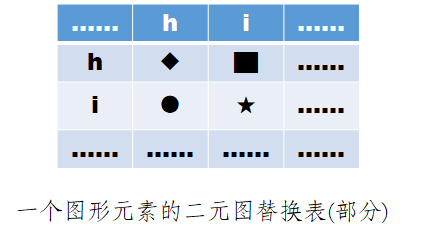
\includegraphics[width=0.6\textwidth]{diagram-example.png}
\end{figure}
\par
***********************************************************\par
\vspace{1cm}

\subsection{单一混合字母表Vigen\`{e}re(Single Mixed Alphabet Vigen\`{e}re )}
先做一个简单的替换,然后做一个Vigen\`{e}re加密。
\[e_i=f(m_i)+k_i\]
\[m_i=f^{-1}(e_i-k_i)\]
\textbf{译者注:此处$e_i$是密文,$m_i$是明文。}
\par

这个系统的“逆”是先做一个Vigen\`{e}re加密,再做一个简单替换。
\[e_i=g(m_i+k_i)\]
\[m_i=g^{-1}(e_i)-k_i\]
\textbf{译者注:这里的“逆”是指颠倒替换和Vigen\`{e}re执行顺序。}\par


\subsection{矩阵系统(Matrix System) \protect\footnote{See L . S . Hill ,“ Cryptography in an Algebraic Alphabet , ” American Math . Monthly ,v. 36 , No. 6 , 1 , 1929, pp. 306 -312 ; also “ Concerning Certain Linear Transformation Apparatus of Cryptography , ” v. 38 , No. 3 , 1931 , pp. 135-154 } }

一种n元替换方法是使用具有逆的矩阵对连续的n个元素进行运算,假设字母编号为0到25,使其成为代数环的元素。根据消息的n元$m_1\ m_2\cdots m_n$,矩阵$a_{ij}$给出n元密文
\[e_i=\sum_{j=1}^{n}a_{ij}m_j\qquad i=1,\cdots,n\]
矩阵$a_{ij}$是密钥,用逆矩阵进行解密。当且仅当行列式$|a_{ij}|$在环中具有逆元素时,逆矩阵将存在。


\subsection{游乐场密码(The Playfair Cipher)}

这是一种特殊类型的二元图替换,将乱序的25个字母写在$5\times 5$的正方形中。(字母J在密码工作中经常被丢弃,因为J很少见,当它出现时,可以用I代替。)假设密钥正方形如下所示:

\begin{equation}
	\begin{array}{ccccc}
	L &Z &Q &C &P\\
	A &G &N &O &U\\
	R &D &M &I &F\\
	K &Y &H &V &S\\
	X &B &T &E &W \nonumber
	\end{array} 
\end{equation}


例如,数字符号AC的替代物是由A和C定义的矩形的其他两个角上的一对字母,即LO,首先取L,因为它在A之上。如果数字符号与RI在一条水平线上,则使用右边DF的字母;RF变为DR。如果字母在垂直线上,则使用它们下面的字母,因此PS变为UW。如果字母相同,则可以使用空值来分隔它们,或者可以省略一个,等等。

\subsection{多重混合字母替换(Multiple Mixed Alphabet Substitution)}
在这个密码中,有一组按顺序使用的d个简单替换。如果周期d是4,
\[m_1m_2m_3m_4m_5m_6\cdots\]
变成
\[\underline{f_1(m_1)f_2(m_2)f_3(m_3)f_4(m_4)}f_1(m_5)f_2(m_6)\cdots\]


\subsection{自动密钥密码(Autokey Cipher)}

这是一种Vigen\`{e}re类型的系统,其中消息本身或生成的密文被用作“密钥”,称为自动密钥密码。加密从“启动密钥”(在我们的意义上是整个密钥)开始,并继续使用消息或密文,其长度被启动密钥的长度所取代,如下所示,其中启动密钥是COMET。消息用作“密钥”:
\begin{equation}
	\begin{aligned}
	Message\qquad    &\uwave{SENDSUP}PLIES\cdots \\
	Key\qquad        &\underline{COMET}\uwave{SENDSUP}\cdots \\
	Crytorgram\qquad &USZHLMTCOAYH\cdots \nonumber
	\end{aligned}
\end{equation}

如果用密文做“密钥”则是:\footnote{从保密的角度来看,这个系统是微不足道的,因为除了开头的d个字母,敌人拥有整个“密钥”.}
\begin{equation}
	\begin{aligned}
		Message\qquad    &SENDSUPPLIES\cdots \\
		Key\qquad        &\underline{COMET}\uwave{USZHLOH}\cdots \\
		Crytorgram\qquad &\uwave{USZHLOH}OSTS\cdots \nonumber
		\end{aligned}
\end{equation}

\subsection{分馏密码(Fractional Ciphers)}

在这种情况下,每个字母首先被加密为两个或多个字母或数字,这些符号以某种方式混合(例如,通过换位)。解密时,结果被重新转换为原始字母表。因此,使用混合的25字母表作为密钥,我们可以通过下表将字母转换为两个五位数字:
\begin{center}
	\begin{tabular}{c|c|c|c|c|c}
		
		& 0 & 1 & 2 & 3 & 4 \\ 
		\hline 
		0&L  & Z & Q & C & P \\ 
		\hline 
		1&A  & G & N & O & U \\ 
		\hline 
		2& R & D &M  & I & F \\ 
		\hline 
		3& K & Y & H & V & S \\ 
		\hline 
		4& X & B & T & E & W \\ 
		
	\end{tabular} 
\end{center}


通过查表B转换为41,以此种方式置换后得到的一系列数字,它们被成对地取出来,并翻译回字母。

\subsection{编码(Codes)}
在编码中,单词(有时是音节)被替换为字母组。有时会对结果应用一种或另一种密码。

\newpage

%---------------------------------------------
%   
%     5.VALUATIONS OF SECRECY SYSTEMS
%
%---------------------------------------------

\section{保密系统的评价(VALUATIONS OF SECRECY SYSTEMS)}

有很多准则可用于评估提出的保密系统,其中最重要的是下面几个方面:

\subsection{保密程度(Amount of Secrecy)}
有些系统是完美的————敌人拦截任何数量的消息后,情况都不会比以前好。其他一些系统虽然给了敌人一些信息,但并不能完成对拦截密文的破解。在各种可以产生唯一解的破解系统中,实现该解决方案的成本和所需拦截消息数量方面存在很大差异。

\subsection{密钥大小(Size of Key )}

密钥必须通过不可截获的方式从发送点发送到接收点。有时这一点必须谨记。因此,希望密钥尽可能小。\footnote{译者注:在传输时希望密钥越小越好,但是为了增加系统的保密程度,通常我们希望密钥越大越好,这里是相互矛盾的,这就要求在实际操作时,需要取一个平衡点。在工程中很多时候,都是要寻找这样一个平衡点的。}

\subsection{加密和解密操作的复杂性(Complexity of Enciphering and Deciphering Operations)}

当然,加密和解密应该尽可能简单。如果人工操作,复杂性会导致时间损失、错误等。如果机械操作,复杂性将导致大型昂贵机器。

\subsection{错误传播(Propagation of Errors)}

在某些类型的密码中,加密或传输中一个字母的错误会导致解密文本中的大量错误。这些错误通过解密操作扩散,导致大量信息丢失和需要频繁重发密文。我们自然希望将这种错误扩散最小化。

\subsection{消息扩展(Expansion of Message)}
在某些类型的保密系统中,消息的大小在经过加密过程后增加了。在试图通过添加许多空值来淹没消息统计特性的系统中,可以看到这种情况,这种情况也出现在使用多个替代的情况下。这种情况也出现在许多“隐藏”( concealment)类型的系统中(通常不是我们定义的保密系统)。

\newpage
%---------------------------------------------
%   
%     6.THE ALGEBRA OF SECRECY SYSTEMS
%
%---------------------------------------------

\section{保密系统代数(THE ALGEBRA OF SECRECY SYSTEMS)}
如果我们有两个保密系统$T$和$R$,我们通常用各种办法将他们组合起来形成一个新的保密系统$S$,如果$T,R$有相同的域(消息空间),我们可以用“加权和”组合:
\[S=pT+qR\]
此处$p+q=1$,该操作首先用概率$p$和$q$进行初步选择,确定使用$T$和$R$中的哪一个,该选择是S密钥的一部分。确定后,按最初定义使用$T$或$R$变换。S的全部密钥必须指定使用T和R中的哪一个以及使用T(或R)变换所需密钥。

如果$T$包含变换$T_1,\cdots,T_m$,其选择的概率为$p_1,\cdots,p_m$,$R$包含变换$R_1,\cdots,R_k$,其选择的概率为$q_1,\cdots,q_k$,那么$S=pT+qR$包含变换$T_1,\cdots,T_m,R_1,\cdots,R_k$,其对应的概率分别为$pp_1,pp_2,\cdots,pp_m,qq_1,qq_2,\cdots,qq_k$。

合成系统的一般表达式为:
\[S=p_1T+p_2R+\cdots+p_mU \qquad \sum p_i=1\]

我们注意到,任何系统$T$都可以写成固定操作的和
\[T=p_1T_1+p_2T_2+\cdots+p_mT_m\]
$T_i$是对应于密钥选择$i$的确定加密操作,其被选择的概率为$p_i$。

组合两个保密系统的第二种方法是采用图\ref{Fig:fig3}表示的“乘积”。假设$T$和$R$是两个系统,$R$的定义域(语言(也就是明文)空间)等同于$T$的值域(密文空间)。然后我们可以首先将$T$应用于我们的语言,然后应用$R$生成加密结果。这给出了一个结果运算S,我们将其写成乘积形式\footnote{译者注:运算顺序为从右到左,$RT\cdot m$,其中$m$是消息,那么运算就是$R\cdot (T \cdot m)$。}
\[S=RT.\]

\begin{figure}[htbp]
	\centering
	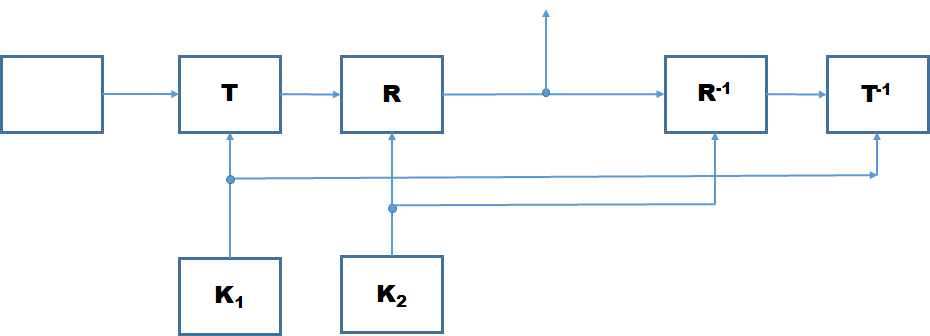
\includegraphics[width=0.8\textwidth]{fig3.png}
	\caption{两个系统的乘积$S=RT$}
	\label{Fig:fig3}
\end{figure}

S的密钥由T和R的两个密钥组成,假设根据它们的原始概率独立地选择。因此,如果选择$T$的$m$个密钥概率分别为:
\[p_1\ p_2\cdots p_m\]
,选择$R$的$n$个密钥的概率为:
\[p'_1\ p'_2\cdots p'_n\]
 ,那么$S$最多具有$mn$个密钥,概率为$p_ip'_j$。在许多情况下,一些乘积变换$R_iT_j$将是相同的,可以组合在一起,增加它们的概率。

乘积加密经常被使用;例如,一种方法是通过换位或维吉尼亚换位进行替换,或者对文本进行编码,并通过替换、换位、分馏(fractionation )等对结果进行加密。

需要注意的是,乘法通常是不可交换的,(我们不总是有RS=SR),尽管在特殊情况下,如替换和换位,它是可交换的。因为它表示一个运算,所以它是可结合的(associative ),即$R(ST)=(RS)T=RST$。此外,我们还有加法加权结合律:
\[p(p'T+q'R)+qS=pp'T+pq'R+qS\]

左右分配律:
\[T(pR+qS)=pTR+qTS\]
\[(pR+qS)T = pRT + qST\]

和
\[p_1T+p_2T+p_3R=(p_1+p_2)T+p_3R\]

应该强调的是,这些加法和乘法的组合运算适用于整个保密系统。两个系统的乘积TR不应与系统中变换的乘积$T_iR_j$混淆,变换乘积也经常出现在本文中。前一个$TR$是保密系统,即一组具有相关概率的变换;后者是一个特殊的变换。此外,两个系统的和$pR+qT$是一个系统,而两个变换的和没有定义。单独的$T_i$和$R_j$不可交换(commute)的情况下,系统$T$和$R$也可以是可交换的,例如,如果R是一个给定周期的Beaufort系统,则所有密钥都是相同的,一般我们有,
\[R_iR_j\neq R_jR_i\]
,当然$RR$不取决于其顺序,实际上,
\[RR=V\]
是有同一周期随机密钥的维吉尼亚密码;另一方面,如果两个系统$T$和$R$的单个$T_i$和$R_j$可交换,则整个系统可交换。

$M$和$E$空间一致的系统,普遍情况是字母序列被转换成字母序列,这称为自同态(endomorphic)。自同态系统$T$可以被提升到$T^n$的幂。

一个保密系统$T$,其与自身的乘积等于T,即
\[TT=T\]
,将被称为幂等(idempotent)。例如,简单替换、周期$p$的换位、周期p的维吉尼亚密码(每个密钥的可能性相等)都是幂等的。

在固定消息空间中定义的所有自同态保密系统的集合构成“代数簇(algebraic variety)”,即一种代数,使用加法和乘法运算。事实上,我们讨论的加和乘的性质可以总结如下:\par

\textsl{具有相同消息空间的一组自同态密码,以及加权加法和乘法的两个组合运算,形成了一个具有单位元素的线性结合代数,并且加权加法中的系数必须是非负的且和为单位元。}

组合操作为我们提供了从某些类型的保密系统构建许多新类型保密系统的方法,正如给出的示例。我们还可以使用它们来描述密码分析员在试图解决未知类型的密码时面临的情况。事实上,他正在解决下面这种类型的保密系统
\[T=p_1A+p_2B+\cdots+p_rS+p'X \qquad \sum p=1\]
其中$A,B,\cdots,S$是已知类型的密码系统,在这种情况下,$p_i$是它们的先验概率,而$p'X$对应于一种全新未知类型密码的概率。

\newpage
%---------------------------------------------
%   
%     7.PURE AND MIXED CIPHERS
%
%---------------------------------------------

\section{纯密码和混合密码(PURE AND MIXED CIPHERS)}

某些类型的密码,如简单替换、确定周期的换位、确定周期的维吉尼亚、混合字母维吉尼亚等(每个密钥都具有相同的可能性),在密钥方面具有一定的同质性。无论密钥是什么,加密、解密过程基本上是相同的。这与下面系统形成对比
\[pS+qT\]
其中S是一个简单的替换,T是一个给定周期的换位。在这种情况下,整个系统根据使用的是替换还是换位而改变加密、解密流程。

这些系统中同质性的原因源于群属性————我们注意到,在上述同质密码的例子中,集合中任何两个变换的乘积$T_iT_j$等于集合中的第三个变换$T_k$。另一方面,$T_iS_j$不等于下面密码系统的任何变换:
\[pS+qT\]
它只包含替换和换位,不包含乘积。

因此,我们可以将\textbf{“纯”密码("pure" cipher)定义为$T_i$构成的一个群(group)。然而,这将过于局限},因为它要求E空间与M空间相同,即系统是自同态的。分馏换位(fractional transposition)与普通换位一样同质,但不是同态的。正确的定义如下:\textbf{如果对于每一个$Ti,Tj,Tk$都存在一个$T_s$,使得
\[T_iT^{-1}_jT_k=T_s\]
并且每个密钥的可能性相等,则此密码系统$T$是纯的。}否则密码系统是混合的。图\ref{Fig:fig2}的系统是混合的。如果所有密钥的可能性相等,则图\ref{Fig:fig4}是纯的。
\footnote{译者注:对于图\ref{Fig:fig4},我们有$T_1,T_2,T_3,T_4$,我们取$T_1,T_2,T_3$,对于$T_1T_2^{-1}T_3$,注意此组合运算是从右到左,中间的逆运算表示从密文空间变换到明文空间,我们取$M_1$验证可知$T_1T_2^{-1}T_3(M_1)=E_2=T_2(M_1)$,依次我们有:\\
$T_1T_2^{-1}T_4=T_3$\\
$T_1T_3^{-1}T_2=T_4$\\
$\ldots$\\
检验所有情况,我们可确定其满足纯系统定义。\par
对于图\ref{Fig:fig2}可知,我们可知对于$M_1$有$T_1T_2^{-1}T_3=T_3$,而对于$M_2$有$T_1T_2^{-1}T_3=T_2$,也就是说,对于不同消息,相同变换组合的等效变换不同,显然这是不满足纯系统定义的。
}

\begin{theorem}
	在纯密码中,将消息空间映射到自身的操作$T^{-1}_i T_j$形成一个群,其秩为$m$,即不同密钥的数量。\footnote{译者注:简单提示,群是满足封闭性、结合律、有单位元、和逆元的二元运算结构。}
\end{theorem}

对于
\[T^{-1}_j T_k T^{-1}_k T_j =  I\]
,每个元素都有一个逆。因为这些运算,结合定律是正确的,群性质遵循:
\[T^{-1}_i T_j T^{-1}_k T_l = T^{-1}_s T_k T^{-1}_k T_l = T^{-1}_s T_l\]
,使用我们的假设,对于一个$s$,$T^{-1}_i T_j= T^{-1}_s T_k$成立。
\par

\vspace{1cm}
\textbf{***********************************************************}\par
\textsl{\textbf{译者注:结合律怎么证的,没看明白!!!}}\par
\textbf{***********************************************************}\par
\vspace{1cm}

当然,$T^{-1}_iT_j$运算意味着用密钥$j$加密消息,然后用密钥$i$解密,这将把我们带回到消息空间。如果$T$是自同态的,即$T_i$本身将空间$\Omega_M$映射为自身(如大多数密码的情况,其中消息空间和密码空间都由字母序列组成),并且$T_i$是一个群,并且有相同可能性,则$T$是纯的,因为
\[T_iT^{-1}_jT_k=T_iT_r=T_s.\]

\begin{theorem}
	两个可交换的纯密码系统的乘积是纯的。
\end{theorem}

如果T和R可交换,那么对于每一个i,j,都有一个适当的l,m,使得$T_i R_j= R_l T_m$,并且\footnote{
	译者注:对于下面的式子推导我们解释如下:\\
	第一个等号,因为$(T_kR_l)^{-1}=R_l^{-1}T_k^{-1}$。\\
	第二个等号,因为可交换,把$R_j$和$R_l^{-1}$交换,$T_k^{-1}$和$T_m$交换,变成纯系统的定义形式。\\
	利用纯系统的定义,规约为两个系统乘积,得到最后一个等式。
}
\begin{equation}
	\begin{aligned}
		T_iR_j(T_kR_l)^{-1}T_mR_n &=T_i R_j R^{-1}_l T^{-1}_k T_m R_n \\
		                          &=R_u R^{-1}_vR_wT_rT^{-1}_sT_i\\
		                          &=R_hT_\sigma
	\end{aligned} 
\end{equation}

然而,交换条件对于乘积是纯密码不是必要的。


只有一个密钥,即只有单个确定操作$T_1$的系统是纯的,因为唯一选择是
\[T_1T^{-1}_1T_1=T_1.\]
因此,将一般密码扩展为这些简单变换的和,也可以将其展现为纯密码的和。

图\ref{Fig:fig4}所示的纯密码示例揭示了某些属性。消息属于某些子集,我们称之为剩余类(residue classes),可能的密文被划分为相应的剩余类。从一个类中的每个消息到对应类中的每一个密文,至少有条连线,不对应的类之间没有连线。类中的消息数是密钥总数的除数。从消息$M$到相应类中密文连线数等于密钥数除以包含消息(或密文)的类中的消息数。附录中显示对于纯密码这通常成立。我们总结为以下定理:

\begin{theorem}\label{source:theorem3}
	在纯系统中,消息可以分为剩余类集合$C_1,C_2,\cdots,C_s$,密文分成对应的剩余类集合$C'_1,C'_2,\cdots,C'_s$,并且具有以下性质:\\
	(1)消息剩余类是互斥的,共同包含所有可能的消息。密文剩余类类似。\\
	(2)使用任何密钥对$C_i$中的任何消息进行加密会在$C'_i$中生成密文。使用任何密钥解密$C'_i$中的任何密文都会生成$C_i$中的消息。\\
	(3)$C_i$中的消息数,记为$\varphi_i$,等于$C'_i$中的密文数,是密钥数$k$的除数。(译者注:也就是说$\varphi_i$是$k$的约数。)\\
	(4)$C_i$中的每条消息都可以通过$k/\varphi_i$个不同密钥加密为$C'_i$中的一个密文。解密类似。
\end{theorem}

\begin{figure}[htbp]
	\centering
	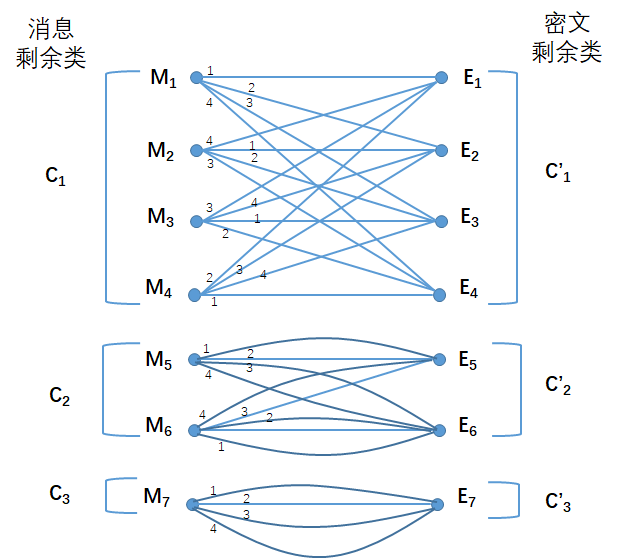
\includegraphics[width=0.6\textwidth]{pure-system.png}
	\caption{"纯"系统}
	\label{Fig:fig4}
\end{figure}

纯密码概念的重要性(以及名称的原因)在于,在纯密码中,所有密钥本质上是相同的。无论对特定消息使用什么密钥,所有消息的后验概率都是相同的。要了解这一点,请注意,应用于同一消息的两个不同密钥会导致同一剩余类$C'_i$中的两个密文。因此,这两个密文可以分别被$\dfrac{k}{\varphi_i}$个密钥解密为$C_i$中的每个消息,而不是其他可能的消息。所有密钥可能性相同时,各消息的后验概率是
\[P_E(M)=\frac{P(M)P_M(E)}{P(E)}= \frac{P(M)P_M(E)}{\sum_M P(M)P_M(E)} =  \frac{P(M)}{P(C_i)}\]
其中$M$在$C_i$中,$E$在$C'_i$中,并且总和是对$C_i$中的所有消息求和。如果$E$和$M$不在相应的剩余类中,则$P_E(M)=0$。类似地,可知不同密钥的后验概率值相同(译者注:用符号表示是$P_E(K)$),但当使用不同密钥时,这些值与不同密钥相关联。$P_E(K)$的同一组值在密钥之间进行了置换。所以,我们有以下结论:

\begin{theorem}
	在纯系统中,各种消息的后验概率$P_E(M)$独立于所选择的密钥。密钥$P_E(K)$的后验概率在值上相同,但进行了不同密钥选择的置换。
\end{theorem}

粗略地说,在纯密码中,任何密钥选择都会导致相同的密码分析问题。由于不同的密钥都导致相同剩余类的密文,这意味着相同剩余类中的所有密文在密码分析上是等价的————它们导致相同的消息后验概率,除了置换之外,密钥的概率也相同。

作为一个例子,所有密钥的简单替换都可能是纯密码。对应于给定密文$E$的剩余类,可通过运算$T_jT^{-1}_K E$,从E获得此剩余类集合中所有密文。在这种情况下,$T_jT^{-1}_k$本身是一个替换,因此$E$上的任何替换都会给出相同剩余类的另一个成员。因此,如果密码是
\[E=X\ C\ P\ P\ G\ C\ F\ Q\]
则
\[E_1=R\ D\ H\ H\ G\ D\ D\ N \]
\[E_2=A\ B\ C\ C\ D\ B\ E\ F \]
等等,都属于同一剩余类。显然,在这种情况下,这些密文本质上是等价的。在使用随机密钥的简单替换中,重要的是字母重复的模式,实际字母是虚拟变量(译者注:dummy variables,也有翻译为“哑变量”)。实际上,我们可以完全省略它们,表明E中的重复模式如下:

\begin{figure}[htbp]
	\centering
	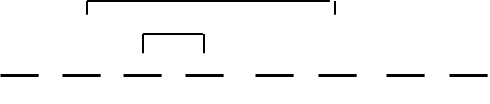
\includegraphics[width=0.6\textwidth]{pattern.png}
\end{figure}

该符号描述了剩余类,但消除了关于类的特定成员的所有信息。因此,它准确地留下了与密码分析相关的信息。这与简单替换密码的一种攻击方法,模式词方法,有关。

在凯撒型密码中,只有密文的mod 26这一个差异是重要的。具有相同$\Delta e_i$的两个密文属于同一剩余类。通过写下消息剩余类的26个成员并挑选出有意义的成员的简单过程,就可以破解这个密码。

具有随机密钥,周期为d的维吉尼亚是纯密码的另一个例子。这里,消息剩余类由所有序列组成,这些序列具有与密文相同的一个差异,以距离$d$分隔字母。对于$d=3$,剩余类定义为:
\[m_1-m_4=e_1-e_4\]
\[m_2-m_5=e_2-e_5\]
\[m_3-m_6=e_3-e_6\]
\[m_4-m_7=e_4-e_7\]
\[\bullet\]
\[\bullet\]
\[\bullet\]

此处$E=e_1,e_2,\cdots$是密文,$m_1,m_2,\cdots$是对应的消息剩余类中的任一消息M。

在具有随机密钥周期d的换位密码中,剩余类由$e_i$的所有排列组成,其中没有$e_i$移出其长度为d的块,距离$d$处的任何两个$e_i$保持在该距离。这用于破译这些密码,如下所示:密文被写入长度为d的连续块中,一个在另一个下面(d=5):\par
\begin{center}
	\begin{tabular}{c c c c c }
		
		$e_1$& $e_2$ & $e_3$ & $e_4$ & $e_5$ \\ 
		
		$e_6$& $e_7$ & $e_8$ & $e_9$ & $e_{10}$ \\ 
		
		$e_{11}$& $e_{12}$ & $\cdot$ & $\cdot$ & $\cdot$ \\ 
		
		$\cdot$& $\cdot$ & $\cdot$ & $\cdot$ & $\cdot$ \\ 
		
	\end{tabular} 
\end{center}

然后将这些列分割并重新排列,以生成有意义的文本。当列被分割时,剩下的唯一信息是密文的剩余类。

\begin{theorem}
	如果$T$是纯密码系统,那么$T_i T^{-1}_j T= T$,此处$T_iT_j$是任意两个$T$的换位变换,相反,如果这对于系统$T$中的任何$T_iT_j$,$T_i T^{-1}_j T= T$成立,则T是纯的。
\end{theorem}

从纯系统的定义来看,这个定理的第一部分是显而易见的。为了证明第二部分,我们首先注意到,如果$T_i T^{-1}_j T= T$,那么$T_i T^{-1}_j T_s$是T的一个变换。所有密钥都是等概率的。我们有$T=\sum_{s}p_sT_s$和
\[\sum_{s} p_sT_iT^{-1}_jT_s = \sum_{s}p_sT_s.\]

左边项的和在$s=j$时结果为$p_jT_i$。右侧只有包含$T_i$的项,所以右侧是$p_iT_i$。由于所有系数都是非负的,因此
\[p_j\leq p_i.\]

当$i,j$互换,相同的讨论也成立,所以有
\[p_j = p_i\]
并且$T$是纯的,$T_iT^{-1}_jT=T$这个条件可以做为纯系统的替代定义。

\newpage
%---------------------------------------------
%   
%     8.SIMILAR SYSTEMS
%
%---------------------------------------------

\section{相似系统(SIMILAR SYSTEMS)}

两个保密系统$R$和$S$被认为是相似的,如果存在具有逆$A^{-1}$的变换$A$,使得
\[R=AS\]

这意味着用$R$加密与用$S$加密相同,因为S加密后,对结果进行$A$变换就是R加密。如果我们用$R\approx S$ 表示“$R$相似于$S$”,那么很明显$R\approx S$意味着$S\approx R$。$R\approx S$和$S\approx T$也意味着$R\approx T$,并且$R\approx R$。这些可以概括为相似性是一种等价关系。

相似性的密码学意义在于,如果$R\approx S$,则从密码分析的角度来看,$R$和$S$是等价的。事实上,如果密码分析员截获了系统$S$中的密文,他只需对其应用转换$A$,就可以将其转换为系统$R$中的密文。系统$R$中的密码通过应用$A^{-1}$转换为$S$中的密文。如果$R$和$S$应用于相同的语言或消息空间,则生成的密文之间存在一对一的对应关系。对应的密文对所有消息给出相同的后验概率分布。

如果有一种破解系统$R$的方法,那么任何相似于$R$的系统$S$都可以被破解,因为S系统可以应用$A$归纳到$R$。这是一种在实际密码分析中经常使用的方法。

作为一个简单的例子,简单替换(其中替换不是字母而是任意符号)类似于使用字母替换的简单替换。第二个例子是凯撒和反向凯撒型密码。后者在破译时,有时会首先转化为凯撒类型,这可以通过颠倒密文中的字母表来实现。当密钥是随机的时,Vigen\`{e}re、Beaufort和变体Beaufort都是相似的,用密钥$K_1 K_2\cdots K_d$初始化的“自动密钥”密码系统(消息用作“密钥”)类似于Vigen\`{e}re类型,密钥以Mod 26方式交替加和减。在这种情况下,对基本密钥一系列dA变换来“解密”自动密钥。

\newpage

\begin{center}
	\section*{第二部分\ 理论保密(THEORETICAL SECRECY)}
\end{center}

%---------------------------------------------
%   
%     9.INTRODUCTION
%
%---------------------------------------------

\section{引言(INTRODUCTION)}

我们现在考虑与系统的“理论保密”有关的问题。\footnote{译者注:原文中,下面的问题并没有分段,为了便于阅读,把问题分成一个个小段落。}\par

当密码分析人员有无限的时间和人力可用于分析密码时,系统对密码分析的免疫性如何?\par

一个密文是否有唯一解(即使它可能需要不切实际的工作量才能找到它),如果没有,它有多少合理的解决方案?\par

在解变得唯一之前\footnote{译者注:在这里唯一的意思是,在破译者看来没有随机性了,明文和密文对应变得唯一。},给定系统必须截取多少文本?\par

无论截获多少加密文本,有没有系统永远不会有求得唯一解的破解系统\footnote{译者注:唯一解就是能确定明文,就是破解的意思。}?\par

是否存在这样的系统,无论截获多少文本,都不会向敌人提供任何信息?\par

在对这些问题的分析中,会用到“通信数学理论”(以下简称MTC)一文中提出的熵、冗余等概念。

\newpage
%---------------------------------------------
%   
%     10.PERFECT SECRECY
%
%---------------------------------------------

\section{完全保密(PERFECT SECRECY)}

让我们假设可能的消息是有限个,$M_1,\ldots,M_n$,并且具有先验概率$P(M_1)$, $\ldots$, $P(M_n)$,这些消息通过$E=T_i M$被加密为可能的密码$E_1,\ldots,E_m$。

密码分析人员截取E,原则上至少可以计算各种消息的后验概率$P_E(M)$,\footnote{译者注:假设我们用的是一个简单替换加密方法,就是用一个字母替换,比如截取到密文“A”,那么对应的明文可能是"A~Z"中的任何一个,每一个明文的可能性都是$\dfrac{1}{26}$,也就是可以得到密文"A"的各个消息的后验概率,$P_{"A"}("A")=\dfrac{1}{26}$,$P_{"A"}("B")=\dfrac{1}{26}$,$P_{"A"}("C")=\dfrac{1}{26}$,\ldots,$P_{"A"}("Z")=\dfrac{1}{26}$。}
可以通过以下条件来定义完全保密性:对于所有E,后验概率等于先验概率,并且这些值相互独立\footnote{译者注:“这些值”指的是这些先验概率。}。在这种情况下,截获消息并没有给密码分析员任何信息\footnote{纯粹主义者可能会反对这一说法,因为敌人获得了一些信息,至少他知道有一条消息被发送了。这可以通过在消息中有一个“空白”对应于“没有消息”来回答。如果没有消息被发送,则该空白将被加密并作为密码发送,那么,即使是这一小部分剩余信息也会被删除。}。任何依赖密文信息的行为都不会被改变,因为所有与密文相关概率都保持不变。反之,如果不是这样,就会出现敌人一定有某个先验概率,某些密钥和信息的选择,因敌人的概率变化而可能发生。这可能会影响他的行动,从而无法获得完全保密。因此,给出的定义是我们对完全保密的直觉。

完全保密的充分必要条件如下:根据贝叶斯公式
\[P_E(M)=\dfrac{P(M)P_M(E)}{P(E)}\]
其中:\\
$P(M)=$消息M的先验概率。\\
$P_M(E)=$如果选择消息M时,密文E的条件概率,也就是,从消息M产生密文E的所有密钥的概率之和。\\
$P(E)=$任何情况下获得密码E的概率。\\
$P_E(M)=$密文E被截获后,消息M的后验概率。\par

对于完全保密系统,对于所有的E和M,$P_E(M)$必须等于$P(M)$。因此,P(M)=0这种情况必须排除,因为我们要求等式成立不依赖于$P(M)$的值,对所有的M和E,
\[P_M(E)=P(E).\]
反过来讲,如果$P_M(E)=P(E)$,那么
\[P_E(M)=P(M),\]
我们获得了完全保密系统。所以我们有以下定理。

\begin{theorem}
	完全保密系统的的充分必要条件是,对于所有M和E,
	\[P_M(E)=P(E).\]
	也就是说,$P_M(E)$必须独立于M。
\end{theorem}

换句话说,对于所有$M_i$、$M_j$和E,将$M_i$转换为给定密文E的所有可能密钥的总概率等于将$M_j$转换为相同E的所有可能密钥的总概率。

现在,E必须和M一样多,因为对于固定的i,$T_i$给出了所有M和某个E之间的一一对应关系。对于完全保密,任何E和任何一个M,$P_M(E)=P(E)\neq 0$。因此,至少有一个密钥将任一M转换为这个E中的一个。但从固定M变换不同E的所有密钥必须不同,因此不同密钥的数量至少与M的数量一样多,仅使用此数量的密钥就可以获得完美的保密性,如下例所示:让$M_i$编号为1到n,$E_i$相同,使用n个密钥,并设
\[T_i M_j=E_s\]
此处$s=i+j \mod(n)$,\footnote{译者注:明文和密钥数量都为n,采用这个式子表达密文也是n个,我们n=3时的两个例子看看:
%下面是一个图
%	\begin{tikzpicture}  
%	[scale=.3,auto=center,every node/.style={circle,fill=blue!20}] 
%	% here, node/.style is the style pre-defined, that will be the default layout of all the nodes. You can also create different forms for different nodes.  
%	
%	\node (m1) at (1,3) {$m_1$};  
%	\node (m2) at (5,3)  {$m_2$}; 
%	\node (m3) at (9,3)  {$m_3$}; 
%	% These all are the points where we want to locate the vertices. You can create your diagram first on a rough paper or graph paper; then, through the points, you can create the layout. Through the use of paper, it will be effortless for you to draw the diagram on Latex.  
%	\node (k1) at (1,0)  {$T_1$};  
%	\node (k2) at (5,0) {$T_2$};  
%	\node (k3) at (9,0)  {$T_3$};  
%	\node (e1) at (1,-3)  {$E_1$};  
%	\node (e0) at (5,-3) {0};  
%	\node (e2) at (9,-3)  {$E_2$};  
%	
%	\node (e3) at (5,-6) {$E_3$};  
%	
%	\draw (m1) -- (k2); % these are the straight lines from one vertex to another  
%	\draw (m2) -- (k3);
%	\draw (m3) -- (k1);
%	
%	\draw (k1) -- (e1);
%	\draw (k2) -- (e0);
%	\draw (k3) -- (e2);
%	
%	\draw (e0) -- (e3);
%	\end{tikzpicture}
%
%	\begin{tikzpicture}  
%	[scale=.3,auto=center,every node/.style={circle,fill=blue!20}] 
%	
%	\node (m1) at (1,3) {$m_1$};  
%	\node (m2) at (5,3)  {$m_2$}; 
%	\node (m3) at (9,3)  {$m_3$}; 
%	
%	\node (k1) at (1,0)  {$T_1$};  
%	\node (k2) at (5,0) {$T_2$};  
%	\node (k3) at (9,0)  {$T_3$};  
%	
%	\node (e0) at (1,-3)  {0};  
%	\node (e2) at (5,-3) {$E_2$};  
%	\node (e1) at (9,-3)  {$E_1$};  
%	
%	\node (e3) at (1,-6) {$E_3$};  
%	
%	\draw (m1) -- (k3); % these are the straight lines from one vertex to another  
%	\draw (m2) -- (k1);
%	\draw (m3) -- (k2);
%	
%	\draw (k1) -- (e0);
%	\draw (k2) -- (e2);
%	\draw (k3) -- (e1);
%	
%	\draw (e0) -- (e3);
%	
%	\end{tikzpicture}
%----------------------
\begin{figure}[H]
	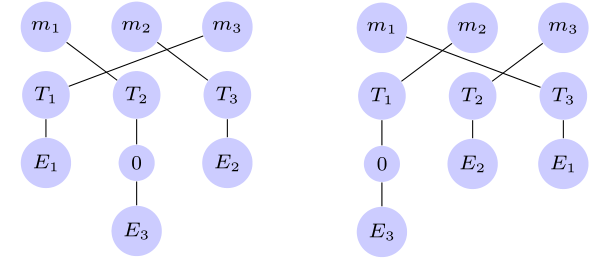
\includegraphics[width=0.6\textwidth]{tran-sample1.png}
\end{figure}
}
在这种情况下,我们有$P_E(M)=\dfrac{1}{n}=P(E)$,具有完全保密性。图\ref{fig:perfect-sys}中所示的列子,$s=i+j-1 \mod(5)$。
\footnote{
	译者注:根据图\ref{fig:perfect-sys},我们有:\\
	\begin{equation}\nonumber
		\begin{aligned}
			&T_1(M_1)=E_1\Rightarrow 1+1-1\mod{5}=1\quad T_2(M_1)=E_2\Rightarrow 2+1-1\mod{5}=2\\
			&T_3(M_1)=E_3\Rightarrow 3+1-1\mod{5}=3\quad T_4(M_1)=E_4\Rightarrow 4+1-1\mod{5}=4\\
			&T_5(M_1)=E_5\Rightarrow 5+1-1\mod{5}=5\\
			&T_5(M_2)=E_1\Rightarrow 5+2-1\mod{5}=1\quad T_1(M_2)=E_2\Rightarrow 1+2-1\mod{5}=2\\
			&T_2(M_2)=E_3\Rightarrow 2+2-1\mod{5}=3\quad T_3(M_2)=E_4\Rightarrow 3+2-1\mod{5}=4\\
			&T_4(M_2)=E_5\Rightarrow 4+2-1\mod{5}=5\\
			&\ldots
		\end{aligned}	
	\end{equation}
}

\begin{figure}[htbp]
	\centering
	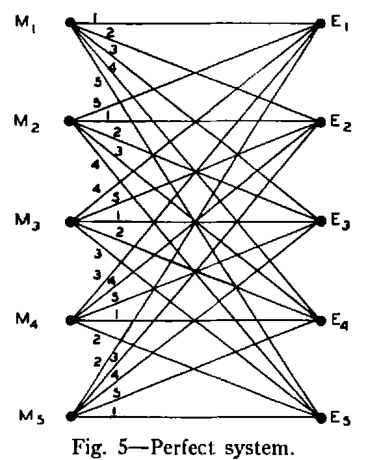
\includegraphics[width=0.6\textwidth]{perfect-sys.png}
	\caption{完全保密系统}
	\label{fig:perfect-sys}
\end{figure}

密文数、消息数和密钥数都相等的完全保密系统具有以下特性:
\begin{enumerate}
	\item 每个M通过一条线与每个E连接。
	\item 所有密钥的可能性相同。
\end{enumerate}
因此,系统的矩阵表示是“拉丁方阵”(Latin Square)\footnote{译者注:拉丁方阵(英语:Latin square)是一种 $n\times n$ 的方阵,在这种 $n\times n$ 的方阵里,恰有 n 种不同的元素,每一种不同的元素在同一行或同一列里只出现一次。拉丁方阵有此名称是因为瑞士数学家和物理学家欧拉使用拉丁字母来做为拉丁方阵里的元素的符号。以下是两个拉丁方阵举例:\\
$\begin{bmatrix}
	1 & 2 & 3\\
	2 & 3 & 1\\
	3 & 2 & 1
\end{bmatrix}$
$\begin{bmatrix}
	a & b & d & c\\
	b & c & a & d\\
	c & d & b & a\\
	d & a & c & b
\end{bmatrix}$
}.


在MTC文章中阐述了信息可以通过熵方便地测量。如果我们有一组概率为$p_1,\ldots,p_n$的可能性,则熵H为:
\[H=-\sum p_i\log{p_i}\]

在保密系统中,涉及两种统计选择,即消息和密钥。我们可以测量选择消息时产生的信息量H(M):
\[H(M)=-\sum P(M)\log{P(M)},\]

以上是所有可能消息的总和。类似地,存在与密钥选择相关的不确定性:
\[H(K)=-\sum P(K)\log{P(K)}.\]

在上述类型的完全保密系统中,消息中的信息量最多为$\log{n}$(当所有消息均为等概率时发生)。只有当密钥不确定性至少为$\log{n}$时,才能完全隐藏该信息。这是经常出现的一般原则的第一个例子:在给定密钥不确定性的情况下,我们所获内容是有极限的,我们可以引入到加密方案中的不确定性不能大于密钥不确定性。

如果消息的数量是无限的,情况就更加复杂了。例如,假设它们是由一个适当的Markoff过程生成的无限个字母序列。很明显,没有一个有限密钥会给出完全保密性。然后,我们假设密钥源以相同的方式生成密钥,也是一个无限符号序列。进一步假设只需要长度$L_K$的密钥来加密和解密长度$L_M$的消息。假设消息字母表中字母数的对数为$R_M$,\footnote{译者注:字母表中字母数为$N_{alphabet}$,$R_M=log N_{alphabet}$。}密钥字母表的对数为$R_K$。然后,从有限情况来看,很明显,完全保密需要
\footnote{译者注:熵最大为$H=-\sum_{i=1}^{n}{\frac{1}{n}\log{\frac{1}{n}}}=\log{n}$,熵是一个平均信息量,也就是每个字母平均信息量,对于某个长度的字母序列,这个序列的信息量(或不确定性)就是长度乘H,所以$R_ML_M$是消息的信息量,$R_KL_K$是密钥的信息量,我们要求密钥的信息量要大于等于消息的信息量,所以有$R_M L_M \leq R_K L_K$。}
\[R_M L_M \leq R_K L_K.\]

Vernam系统是这种类型的完全保密系统的一个具体实现。

这些结果是根据消息的未知性或随意性,也就是消息的先验概率推导出来的。完全保密所需的密钥取决于可能消息的总数。

人们可以预期,如果消息空间具有固定的已知统计信息,从而在MTC文章中表述的意义上,具有确定生成信息的平均速率R,那么所需的密钥量可以平均以这个比率$\dfrac{R}{R_M}$减少,\footnote{译者注:消息熵为$R_M$,而且我们已知$R_M\leq R_K$,当消息熵变为R时,也就是减少了$\dfrac{R}{R_M}$,那么密钥熵同比例减少,不影响系统的完全保密性,也就是$\dfrac{R}{R_M}\times R_M\leq \dfrac{R}{R_M}\times R_K$。}这确实是正确的。事实上,消息可以通过一个变换器传递,该变换器消除了冗余,并以该比率减少预期长度,在Vernam系统中可应用此结果。很明显,每个消息字母使用的密钥数量在统计上减少了一个因子$\dfrac{R}{R_M}$,在这种情况下,密钥源和信息源刚好匹配————1bit密钥完全隐藏了1bit消息信息。MTC中使用的方法也很容易获得,这是可以做到最好的情况,MTC文中也使用了这个方法。

完全保密系统在实际情况中占有一席之地————它们可以在最重视完全保密的情况下使用,例如,最高级别指挥之间的通信,或者在可能的消息数量很少的情况下。因此,举一个极端的例子,如果只预期到两条消息“是”或“否”,那么一个完全系统是适合的,可能的转换表\footnote{译者注:原文中的表不是很清楚,从辨识出来的结果看,不太容易理解,应该是指的结果在两个密钥下的加密结果,应该这样表述也许更清楚些:\\
\begin{tabular}{|c|c|c|}
	\hline 
	M\qquad &K=A &K=B \\ 
	\hline 
	yes& 0 & 1 \\ 
	\hline 
	no& 1 & 0 \\ 
	\hline 
\end{tabular} \\
另外,我么也可以猜测,可能在第一个单元格中,M和K之间有个斜线。
}
:
\begin{center}
	\begin{tabular}{|c|c|c|}
		\hline 
		M\qquad K& A & B \\ 
		\hline 
		yes& 0 & 1 \\ 
		\hline 
		no& 1 & 0 \\ 
		\hline 
	\end{tabular} 
\end{center}


当然,对于大型通信系统来说,完全保密系统的缺点是必须发送相当数量的密钥。在接下来的章节中,我们将考虑使用较小的密钥空间可以实现什么,特别是使用有限的密钥。

\newpage
%---------------------------------------------
%   
%     11.EQUIVOCATION
%
%---------------------------------------------

\section{疑义度(EQUIVOCATION)}

让我们假设一个简单的用于英语文本的替换密码,我们截取了N个字母长度的加密文本。当N相当大时,比如50个以上的字母,密码几乎总是有唯一解;也就是说,有一个正常的英语序列,通过简单的替换转换为截取的素材。然而,N越小,出现一个以上解决方案的可能性越大;当N=15时,通常会有相当多的可能的文本片段适合\footnote{译者注:“适合”是指有相当多的正常英文序列可以通过简单替换对应到截取的密文上。},而当N=8时,所有长度的合理英语序列中的一个很大部分(大约1/8)是可能的答案,因为在8个字母中很少有一个以上的重复字母。当N=1时,任何字母都是明显可能的,并且具有与先验概率相同的后验概率,所以对于一个字母,系统是完全保密的。

这通常发生在可破解密码中。在截取任何材料之前,我们可以想象各种可能的消息以及各种密钥所附带的先验概率。当材料被截取时,密码分析员计算后验概率;随着N的增加,某些消息的概率会增加,但是大多数消息的概率都会减少,直到最后只剩下一条消息,这条消息的概率几乎为1,而所有其他消息的总概率几乎为零。

这种计算实际上可以在非常简单的系统中进行。表I显示了应用于英语文本的凯撒型密码的后验概率,其中密钥从26种可能中随机选择。为了能够使用标准字母、连续两字母和三字母频率表,文本是从一个随机的点开始的(如打开一本书,拿支铅笔随机点下去)。以这种方式从“creases to…”开始,依次往后。如果已知该信息是一个句子开始,则必须使用一组不同的概率,对应于句子开头字母、两字母等的频率。

\begin{center}
	{TABLE I\\一个Caesar类型加密系统的后验概率}
	\begin{tabular}{|c|c|c|c|c|c|}
		\hline 
		解密& N=1 & N=2 & N=3 & N=4 & N=5  \\ 
		\hline 
		C R E A S& . 028 & .0377 & .1111 & .3673 & 1 \\ 
		\hline 
		D S F B T& . 038 & .0314 &  &  &  \\ 
		\hline 
		E T G C U& . 131 & .0881 &  &  &  \\ 
		\hline 
		F U H D V& . 029 & .0189 &  &  &  \\ 
		\hline 
		G V I E W& .020  &  &  &  &  \\ 
		\hline 
		H W J F X& .053 & .0063 &  &  &  \\ 
		\hline 
		I X K G Y& .063 & .0126 &  &  &  \\ 
		\hline 
		J Y L H Z& .001 &  &  &  &  \\ 
		\hline 
		K Z M I A& .004 &  &  &  &  \\ 
		\hline 
		L A N J B& .034 & .1321 & .2500 &  &  \\ 
		\hline 
		M B O K C& .025 &  & .0222 &  &  \\ 
		\hline 
		N C P L D& .071 & .1195 &  &  &  \\ 
		\hline 
		O D Q M E& .080 & .0377 &  &  &  \\ 
		\hline 
		P E R N F& .020 & .0818 & .4389 & .6327 &  \\ 
		\hline 
		Q F S O G& .001 &  &  &  &  \\ 
		\hline 
		R G T P H& .068 & .0126 &  &  &  \\ 
		\hline 
		S H U Q I& .061 & .0881 & .0056 &  &  \\ 
		\hline 
		T I V R J& .105 & .2830 & .1667 &  &  \\ 
		\hline 
		U J W S K& .025 &  &  &  &  \\ 
		\hline 
		V K X T L& .009 &  &  &  &  \\ 
		\hline 
		W L Y U M& .015 &  & .0056 &  &  \\ 
		\hline 
		X M Z V N& .002 &  &  &  &  \\ 
		\hline 
		Y N A W O& .020 &  &  &  &  \\ 
		\hline 
		Z O B X P& .001 &  &  &  &  \\ 
		\hline 
		A P C V Q& .082 & .0503 &  &  &  \\ 
		\hline 
		B Q D Z R& .014 &  &  &  &  \\ 
		\hline 
		H ( 十进制数 )& 1.2425 & .9686 & .6034 & .285 & 0 \\ 
		\hline 
	\end{tabular} 
\end{center}

具有随机密钥的凯撒密码是一种纯密码,选择某个密钥不影响后验概率。要确定这些概率,我们只需列出所有密钥的可能解密,并计算它们的先验概率。后验概率是这些先验概率除以它们的和。这些可能的解密是通过以下标准过程找到的:从消息中“顺着字母表往下走”,在Table I左边列出,这些构成了消息的剩余类。截取一个字母时,后验概率等于字母的先验概率\footnote{该表的概率取自Fletcher Pratt在1939年纽约Blue Ribbon Books出版的《 Secret and Urgent  》一书中给出的频率表。虽然不完整,但它们足以满足当前的目的。},并显示在标题为N=1的列中。截取两个字母时,概率是调整为
和为1的双字母概率(译者注:也就是归一后的双字母概率),如N=2列所示。

三字母出现频次也已统计制成表格,查表计算结果见N=3列所示。对于四个和五个字母的序列概率,可通过与三字母频次相乘粗略获得,
\[p(ijkl)=p(ijk)p_{jk}(l).\]

请注意,在三个字母的情况下,该字段已缩小到四个概率相当高的消息,其他消息概率相对较小。在四个字母时有两种可能性,在五个字母时只有一种正确的破译。(\textbf{译者注:Table I 表中概率的计算过程,见译者加的附录“译者注附录:Table I的计算”})

原则上,这可以用任何系统,但是,只能是在密钥非常小的情况,否则可能的数量非常大,这妨碍了实际的计算。

这组后验概率描述了密码分析员如何随着加密材料的获得,对消息和密钥的了解逐渐变得更加精确。然而,对于我们的目的来说,这一描述过于复杂且难以获得。所期望的是对这种方法的简化描述,以获得可能实现的唯一解决方案。

当传输信号受到噪声干扰时,通信理论中也会出现类似的情况。在只知道接收信号给出的扰动版本时,有必要对实际传输的不确定性进行适当的度量。在MTC中,当接收信号已知时,这种不确定性的自然数学度量是发送信号的条件熵。为了方便起见,这个条件熵被称为疑义度(equivocation)\footnote{译者注:equivocation的翻译借鉴\url{https://baike.baidu.com/item/}信道疑义度,但是在西安电子科技大学王育民老师的ppt中,被翻译为“含糊度”}。

从密码分析者的角度来看,保密系统与嘈杂的通信系统几乎相同。消息(传输的信号)通过一个统计元件,即加密系统,通过经过统计选择的密钥来操作。此操作的结果是可用于分析的密文(类似于扰动信号)。这两种情况的主要区别是:首先,加密变换的操作通常比信道中的扰动噪声更复杂;其次,保密系统的密钥通常是从有限的可能性集合中选择的,而信道中的噪声更经常地连续引入,实际上是从无限集合中选择的。

考虑到这些因素,很自然地将疑义度作为理论上的保密指标。可以注意到,有两个重要的疑义度,即密钥和消息。它们分别由$H_E(K),H_E(M)$表示:
\[H_E(K)=\sum_{E,K}{P(E,K)\log{P_E(K)}}\]
\[H_E(M)=\sum_{E,M}{P(E,M)\log{P_E(K)}}\]
其中,E、M和K是密文、消息和密钥,并且:\\
$P(E,K)$是密钥K和密文E的概率\\
$P_E(K)$是密钥K的后验概率,如果密文E被截获\\
$P(E,M)$和$P_E(M)$使用消息替换密钥后相似的概率\\

$H_E(K)$的和是一定长度(例如N个字母)下,的所有可能密文和所有密钥的总和。对于$H_E(M)$,总和是长度为N的所有消息和密文。因此,$H_E(K)$和$H_E(M)$都是N的函数,即截获的字母数。有时会用$H_E(K,N)$和$H_E(M,N)$来明确表示。请注意,这些都是“全部”疑义度;即,我们不除以N来获得MTC中使用的疑义度率。\footnote{译者注:$H_E(K)$是知道密文时,密钥的平均信息量。}

在通信理论中,关于疑义度作为不确定性度量的讨论也适用于此。我们注意到,零疑义度要求一条消息(或密钥)具有单位概率,其他概率都为零,此消息对应于完整的知识。看做N的函数,疑义度的逐渐减少对应于原始密钥或消息的知识的增加。绘制两条疑义度曲线,N的函数,这被称为所讨论的保密系统的疑义度特征(equivocation characteristics )。


上面考虑的凯撒型密码的$H_E(K,N)$和$H_E(M,N)$值已经计算出来,并在Table I的最后一行给出。在这种情况下$H_E(K,N)$和$H_E(M,N)$是相等的,并以十进制数字给出(即,在计算中使用对数基数10)。应该注意,这里的疑义度是针对特定密文的,也就是说和是基于M(或K)而不是E,通常,总和将覆盖长度为N的所有可能截获的密文,并给出平均不确定性。对于这种一般计算来说,计算困难是令人望而却步的。

\vspace{1cm}
*********************************************\par
译者注:这里所说的$H_E(K,N)$和$H_E(M,N)$值不知道在表中对应最后一行哪个?怎么计算的也没看明白!\par
*********************************************\par
\newpage
%---------------------------------------------
%   
%     12.PROPERTIES OF EQUIVOCATION
%
%---------------------------------------------

\section{疑义度性质(PROPERTIES OF EQUIVOCATION)}

疑义度被证明具有许多有趣的特性,其中大多数都符合我们的直观理解。我们将首先证明,当截获更多的加密材料时,密钥或消息某(固定)部分的疑义度在减少。

\begin{theorem}
	密钥的疑义度$H_E(K,N)$是N的非递增函数,消息的前A个字母的疑义度是被截获的字母数N的非递增函数。如果截获了N个字母,则消息的前N个字母的疑义度小于或等于密钥的疑义度。这可以写为:\\
	$H_E(K,S) \leq H_E(K,N) \qquad S\geq N$\\
	$H_E(M,S) \leq H_E(M,N) \qquad S\geq N$(H 是文本前A个字母疑义度)\\
	$H_E(M,N) \leq H_E(K,N)$
\end{theorem}

定理第二个结果中关于前A个字母的限定条件是,不会根据截获的消息量来计算疑义度。如果是,消息疑义度可能会(而且通常会)增加,这仅仅是因为更多的字母代表了更大的可能范围的信息。定理的结果是我们希望依据一个好的保密指标(index)得到结果,因为我们很难预期在截获额外材料后平均情况会比以前更糟。可以被证明的事实为我们使用疑义度度量提供了进一步的理由。

该定理的结果是MTC中证明的条件熵的某些性质的结果。因此,为了证明定理7的第一个或第二个陈述,我们对任何偶然事件A和B都有
\[H(B)\geq H_A(B).\]

如果我们用密钥替换B(知道密文的前S个字母),用N和S之差替换A,我们会得到第一个结果。\footnote{译者注:我们按定理中的条件,$S\geq N$,那么$A=S-N$,如果把N,S和A都看成密钥长度,就是说长度为A的密钥后续长度为N的密钥,拼接成为长度为S的密钥。$H(B)\geq H_A(B)$,这个式子用自然语言来描述就是:事件B的疑义度大于等于(不小于)在事件A发生情况下,事件B的疑义度。我们把B看成密钥,上面这句话可以说成:密钥长度为N的密钥疑义度大于等于(不小于)在密钥长度为S的密钥疑义度,因为密钥S是两个事件先后的发生,可以写为:$H(K,N)\geq H(K,S)$}
同样,用消息替代B会得到第二个结果\footnote{译者注:这个推理过程和密钥的类似,消息长度为S,可以看成是长度为A和N的消息拼接,$S\geq N,A=S-N$,那么S事件可以看成是先发生A事件,再发生N事件,也就是$H(M,N)\geq H(M,S)$。}。
最后一个结果来自\footnote{译者注:注意下面这个式子里的$H_{E}(K,M)$和上面式子里的$H_{E}(K,S)$不是同一个意思,$H_{E}(K,M)$表示随机变量K和M的联合熵,或,联合疑义度,而$H_{E}(K,S)$是一种标记方法,表示长度为S的密钥K疑义度。根据联合熵的定义,我们有$H(XY)=H(X)+H(Y|X)=H(Y)+H(X|Y)$,所以有$H_E(M) \leq H_E(K,M) $。}
\[H_E(M) \leq H_E(K,M) = H_E(K) + H_{E,K}(M)\]
并且,由于K和E唯一决定M,所以有$H_{E,K}(M)=0$。\footnote{译者注:那么我们有$H_E(M) \leq H_E(K,M) = H_E(K) + H_{E,K}(M)\Rightarrow H_E(M) \leq H_E(K)$。}

由于消息和密钥是独立选择的,所以我们有
\[H(M,K)=H(M)+H(K).\]

进一步有,
\[H(M,K)=H(E,K)=H(E)+H_E(K),\]
上式的第一个等号由M和K或E和K的知识等同于所有三者的知识这一事实产生。结合这两者,我们得到了密钥疑义度公式:
\[H_E(K)=H(M)+H(K)-H(E).\]

特别地,如果$H(M)=H(E)$,则密钥$H_E(K)$的疑义度等于密钥的先验不确定性$H(K)$。这发生在上述完全保密系统中。

可以通过类似的方法找到一个消息疑义度的公式。我们有:
\[H(M,E)=H(E)+H_E(M)=H(M)+H_M(E)\]
\[H_E(M)=H(M)+H_M(E)-H(E)\]

如果我们有一个乘积系统$S=TR$,预计第二个加密过程不会减少消息的疑义度。这实际上是真的,可以如下所示:设$M,E_1,E_2$分别为消息和第一个和第二个密码系统。那么:
\[P_{E_1 E_2}(M)=P_{E_1}(M)\]

可得:
\[H_{E_1 E_2}(M)=H_{E_1}(M)\]

因为,对于任何随机变量(chance variables),$x,y,z,H_{xy}(z)\leq H_y(z)$,我们有期望的结果,$H_{E_2}(M) \geq H_{E_1}(M)$。
\footnote{译者注:我们有$H_{E_1E_2}(M)\leq H_{E_2}(M)$,根据前面的结果有$H_{E_1 E_2}(M)=H_{E_1}(M)$,所以可推得$H_{E_1}(M) \leq H_{E_2}(M)$。}

\begin{theorem}
	乘积系统$S=TR$的消息疑义度不小于仅使用$R$时的疑义度。
\end{theorem}

假定我们现在有一个系统T,其可以写成几个系统$R,S,\ldots,U$的加权和:
\[T=p_1 R+p_2 S+\ldots+p_m U \quad \sum {p_i}=1\]

并且系统$R,S,\ldots,U$的疑义度为$H_1,H_2,H_3,\ldots,H_m$.

\begin{theorem}
	加权和系统的疑义度H满足以下不等式:
	\[\sum {p_i H_i} \leq H \leq \sum {p_i H_i} -\sum {p_i\log{p_i}}.\]
	这些是可能的最佳限制。H可能是密钥或消息的疑义度。
\end{theorem}

例如,在分解为简单变换的强理想系统(将在后面描述)中,可以达到以上定理的上限。如果所有系统$R,S,\ldots,U$属于完全不同的密文空间,则达到下限。这一定理可由疑义度的一般不等式
\[H_A(B)\leq H(B) \leq H(A)+H_A(B).\]
来证明。

我们用A表示所使用的特定系统,用B表示密钥或消息。

语言的加权和有一个类似的定理。为此,我们用A表示特定的语言。

\begin{theorem}
	假定一个系统可以被应用于语言$L_1,L_2,\ldots,L_m$,并且有疑义度特征$H_1,H_2,\ldots,H_m$。当应用加权和$\sum {p_i L_i}$,疑义度H的界为:
	\[\sum {p_i H_i} \leq H \leq \sum {p_i H_i}-\sum {p_i \log{p_i}}\]
	这些限制是最好的可能性,所讨论的疑义度可以是密钥的,也可以是消息的。
\end{theorem}

N个消息字母的总冗余$D_N$定义为:
\[D_N=\log{G} -H(M)\]
其中G是长度为N的消息的个数,$H(M)$是从这些消息中任选一个的不确定性。在保密系统中,可能的密文总数等于长度为N的可能消息数,$H(E)\leq \log{G}$。我们有:\\
$\begin{matrix}
	H_E(K) & =H(K)+H(M)-H(E)\\
	       & \geq H(K)- [\log{G}-H(M)].
\end{matrix}$

因此:
\[H(K)-H_E(K)\leq D_N.\]

这表明,例如,在一个封闭系统中,在截获N个字母后,密钥疑义度的减少不大于语言中N个字母的冗余度。在这种包含大多数密码的系统中,只有原始消息中存在冗余才有可能解决问题。

现在假设我们有一个纯系统。假设消息的不同剩余类是$C_1,C_2,C_3,\ldots,C_r$,密文的相应剩余类集是$C_i',C_2',\ldots,C_r'$。$C_i'$中每个E的概率是相同\footnote{译者注:在原文中,此句话中通过辨识是$C_1'$,结合前后文,应该是笔误,应该是$C_i'$,故翻译时翻译为$C_i'$。}:
\[P(E)=\dfrac{P(C_i)}{\varphi_i}\quad \text{E a member of} C_i\]
其中$\varphi_i$是$C_i$中不同消息的个数,所以,我么有:\\
$\begin{matrix}
H(E) & = -\sum_{i}{\varphi_i \dfrac{P(C_i)}{\varphi_i} \log{\dfrac{P(C_i)}{\varphi_i}}}\\
     & = -\sum {P(C_i)\log{\dfrac{P(C_i)}{\varphi_i}}} 
\end{matrix}$

我们在方程$H_E(K)$中做替换,我们得到以下定理。

\begin{theorem}
	对于一个纯密码系统有:
	\[H_E(K) = H(K) + H(M) + \sum_{i} {P(C_i)\log{\dfrac{P(C_i)}{\varphi_i}}}\]
\end{theorem}

在某些情况下,这个结论可以被用来计算$H_E(K)$。

\newpage
%---------------------------------------------
%   
%     13.EQUIVOCATION FOR SIMPLE SUBSTITUTION ON A TWO LETTER LANGUAGE
%
%---------------------------------------------

\section{双字母语言中简单替换的疑义度(EQUIVOCATION FOR SIMPLE SUBSTITUTION ON A TWO LETTER LANGUAGE)}

现在,我们计算简单替换应用于两个字母语言时(译者注:两字母语言就是只有“0”和“1”的情况。),密钥或消息的疑义度,“0”和“1”的概率分别为p和q,并且连续字母独立选择。我们有:
\[H_E(M)=H_E(K)=-\sum {P(E)P_E(K)\log{P_E(K)}}\]

E在特定排列中恰好包含s个“0”的概率为:
\[\dfrac{1}{2} (p^s q^{N-s}+q^s p^{N-s})\]
并且恒等置换和反转置换(系统中仅有的两个)的后验概率分别为:
\[P_E(0)=\dfrac{p^s q^{N-s}}{(p^s q^{N-s}+q^s p^{N-s})}\]
\[P_E(1)=\dfrac{p^{N-s}q^s}{(p^s q^{N-s} + q^s p^{N-s})}\]

对于每个s有$\begin{pmatrix}
N\\
s
\end{pmatrix}$个表达(terms),所以有
\[H_E(K,N) = -\sum_{s} \begin{pmatrix}
N\\
s\end{pmatrix} p^s q^{N-s} \log{\dfrac{p^s q^{N-s}}{(p^s q^{N-s}+q^s p^{N-s})}}.\]

对于$p=\frac{1}{3},q=\frac{2}{3}$和$p=\frac{1}{8},q=\frac{7}{8}$,$H_E(K,N)$的计算如图\ref{fig:fig6}所示。


\begin{figure}[H]
	\centering
	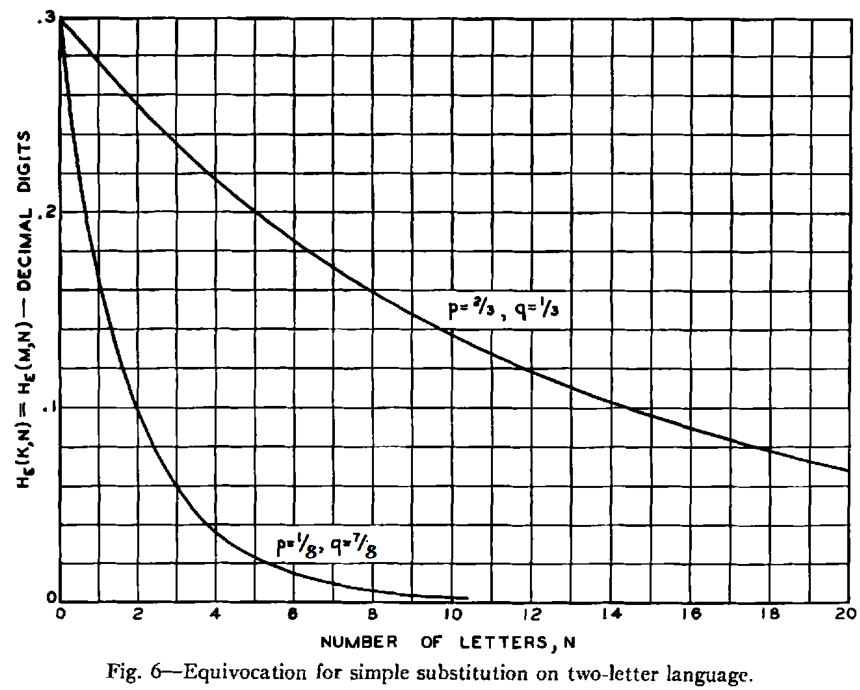
\includegraphics[width=0.8\textwidth]{fig6.png}
	\caption{双字母语言中简单替换的疑义度}
	\label{fig:fig6}
\end{figure}


\newpage
%---------------------------------------------
%   
%     14.THE EQUIVOCATION CHARACTERISTIC FOR A RANDOM CIPHER
%
%---------------------------------------------

\section{随机密码的疑义度特征(THE EQUIVOCATION CHARACTERISTIC FOR A RANDOM CIPHER)}

在上一节中,我们已经计算了两个字母语言简单替换的疑义度。这是关于最简单的密码类型和可能的最简单的语言结构,这些公式太过复杂,几乎毫无用处。我们该如何处理一些实际案例,比如说,英语统计结构极其复杂,分馏密码应用于英语的情况?这种复杂性本身就暗示了一种方法,足够复杂的问题通常可以通过统计来解决,为了利用这一点,我们定义了“随机”密码的概念。

我们做出如下假设:
\begin{enumerate}
	\item 长度为N的可能消息数是$T=2^{R_0 N},R_0=\log_2{G}$,此处G是在字母表中字母的个数,长度为N的可能的密文数也假设为T。
	\item 长度为N的可能消息可以被分为两组,一组先验概率高且相当均匀,另一组总概率可以忽略。高概率组包括$S=2^{RN}$个消息,此处$R=H(M)/N$,也就是说,R是消息源每个字符的平均熵。
	\item 如图2和图4所示,解密操作可以被看作是一系列连线,从每个E映射到不同M。我们假设有$k$个不同的等概率密钥,因此每个E将有$k$条映射线路。对于随机密码,我们假设每个E映射到可能消息的线路随机选择。实际上,随机密码是密码的整体效果,疑义度是这个整体的平均疑义度。
\end{enumerate}

密钥的疑义度定义为:
\[H_E(K)=\sum {P(E) P_E(K) \log{P_E(K)}}.\]

恰好有m个映射(连线)从特定E返回到高概率消息组的概率为:
\[
\begin{pmatrix}
k\\
m
\end{pmatrix}\left(\frac{S}{T}\right)^m \left(1-\frac{S}{T}\right)^{k-m}
\]

如果截获了一个具有m个这种连线的密文,则疑义度为$\log{m}$。这种密文的概率为$\dfrac{mT}{SK}$,因为它可以由m个密钥从高概率消息中产生,每个消息具有概率$\dfrac{T}{S}$,因此疑义度为:
\[H_E(K) = \dfrac{T}{Sk} \sum_{m=1}^{k} \begin{pmatrix}
k\\
m
\end{pmatrix} \left(\dfrac{S}{T}\right)^m \left(1-\dfrac{S}{T}\right)^{k-m} m \log{m} \]

当k较大时,我们希望找到一个简单的近似值。如果m的期望值,即$\overline{m}=Sk/T$,远远大于1,则在二项式分布假设较大值的范围内,$\log{m}$的变化将很小,我们可以用$\log{\overline{m}}$代替$\log{m}$。这现在可以从求和中扣除,然后减为$\overline{m}$。因此,在这种情况下,
\begin{align*}
	&H_E(K) \approx \log{\dfrac{Sk}{T}} =\log{S}- \log{T}+\log{k}\\
	&H_E(K) \approx H(K)-DN,
\end{align*}


此处D是原语言每个字符的平均冗余($D=D_N/N$)。

如果$\overline{m}$与大的$k$相比很小,那么二项式分布可以用泊松分布来近似:

\[\begin{pmatrix}
k\\
m
\end{pmatrix}p^m q^{k-m} \approx \dfrac{e^{-\lambda} \lambda^m}{m\text{!}}
\]

此处$\lambda = \dfrac{Sk}{T}$,因此
\[H_E(K)\approx \dfrac{1}{\lambda} e^{-\lambda} \sum_{2}^{\infty} {\dfrac{\lambda^m}{m\text{!}}m \log{m}}.\]

如果我们用$m+1$代替$m$,可得:
\[H_E(K)\approx  e^{-\lambda} \sum_{1}^{\infty} {\dfrac{\lambda^m}{m\text{!}} \log{(m+1)}}.\]

这可以用于$\lambda$接近于1的区域。对于$\lambda \ll 1$,系列中唯一重要的项是$m=1$;忽略其他的,我们有:\\
\begin{align*}
H_E(K) &\approx  e^{\lambda}\lambda \log{2}\\
       &\approx  \lambda \log{2}\\
       &\approx  2^{-ND}k \log{2}.
\end{align*}


总结:$H_E(K)$看做是截获的字符数N的函数,当N=0时,函数值为H(K),它在$N=\dfrac{H(K)}{D}$附近以斜率$-D$线性下降。在一个短暂的过渡区之后,如果D以每字母比特为单位测量,则$H_E(K)$跟随“半衰期”距离$\frac{1}{D}$的指数函数,大致曲线如图7所示。

通过类似的论证,可以计算出消息的疑义度,是:
\begin{align*}
	&H_E(M) = R_0 N \text{ for } R_0N \ll H_E(K)\\
	&H_E(M) = H_E(K) \text{ for } R_0N \gg H_E(K)\\
	&H_E(M) = H_E(K)-\varphi(N) \text{ for } R_0N \sim H_E(K)
\end{align*}


此处$\varphi(N)$是图7显示的方程,N刻度减少了$\dfrac{D}{R_0}$倍,所以$H_E(M)$以斜率$R_0$线性上升,直到他几乎相交与$H_E(K)$这条线,圆形过渡后,它沿着$H_E(K)$曲线向下。

\begin{figure}[htbp]
	\centering
	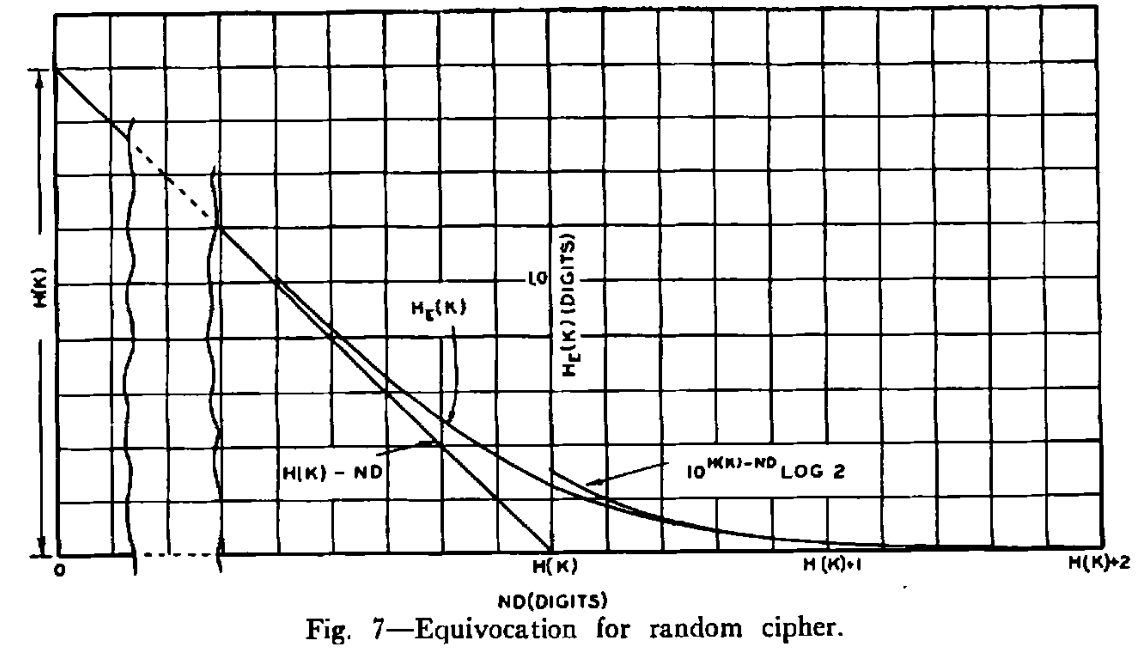
\includegraphics[width=0.9\textwidth]{fig7.png}
	\caption{随机密码的疑义度}
	\label{fig:fig7}
\end{figure}

从图7中可以看出,疑义度的曲线非常尖锐地接近于零。因此,我们可以几乎没有歧义地说解变成唯一。这个字母数被称为唯一解距离(unicity distance)。对于随机密码,它大约为$H(K)/D$。

\newpage
%---------------------------------------------
%   
%     15.APPLICATION TO STANDARD CIPHERS
%
%---------------------------------------------

\section{标准密码的应用(APPLICATION TO STANDARD CIPHERS)}

大多数标准密码涉及相当复杂的加密和解密操作。此外,自然语言的统计结构极其复杂。因此,可以合理地假设,随机密码推导的公式可以应用于这种情况。然而,在某些情况下,必须采取某些纠正措施。需要注意的要点如下:
\begin{enumerate}
	\item 对于随机密码,我们假设密文的可能解密是从可能的消息中随机选择的。虽然在普通系统中严格来说不是这样,但随着加密操作和语言结构的复杂性增加,这种情况变得越来越接近。对于换位密码,很明显,在解密操作下,字母频率被保留了下来。这意味着可能的解密是从一个更有限的组中选择,而不是整个消息空间,并且公式应该变化。有人用$R_1$来代替$R_0$,$R_1$是具有独立字母但有常规字母频次的语言熵速率。在其他一些情况下,可以看到解码趋向于高概率消息的明确趋势。如果没有明显的这类倾向,且系统相当复杂,则使用随机密码分析是合理的。
	\item 在许多情况下,完整密钥不用于加密短消息。例如,在简单的替换中,只有相当长的消息包含字母表中的所有字母,因此涉及完整密钥。
	显然,在这种情况下,随机假设不适用于小N,因为密钥在字母中的区别并未都出现在密文中,这导致分析时出现相同消息,密钥不是随机分布的。
	通过利用“密钥表现特征”,可以很容易获得一个不错的近似值。对于特定的N,可根据密文长度预测有效密钥量,对于大多数密码,这很容易估计。
	\item 由于消息的确定性开始,会产生与随机特征不同的“结束效应”。如果我们在英语文本中随机选取一个起始点,第一个字母(当我们没有观察到前面的字母时)概率是任何普通字母概率。下一个字母更明确,因为我们有双字母频次统计,可能的选择会持续下降。
	选择值的这种下降会持续一段时间。这对曲线的影响是,直线部分被曲线替换,曲线的逼近程度取决于语言的统计结构在相邻字母上的分布程度。做为第一次近似,通过将线移动到半冗余点而修正曲线,如此处语言字母冗余是最终一半时的数。
\end{enumerate}

如果考虑到这三种影响,可以对疑义度特征和唯一解点进行合理估计。如图8所示,可以用图形进行计算。绘制密钥表现特征和总冗余曲线$D_N$(通常由线$ND_{\infty}$完全表示)。它们在交点附近的不同之处在于$H_E(M)$,在英语中应用了一个简单的替换密码,该计算如图9所示的曲线。通过计算N个字母在典型英语段落中出现的频次,来估计这种情况下的关键外观特征。就简单替代的实验数据而言,与图9的曲线非常吻合。例如,实验表明,在大约27个字母处的唯一解点位于极限20和30之间。对于30个字母,这种类型的密码几乎总是有唯一的解决方案,而对于20个字母,通常很容易找到许多解决方案。

\begin{figure}[htbp]
	\centering
	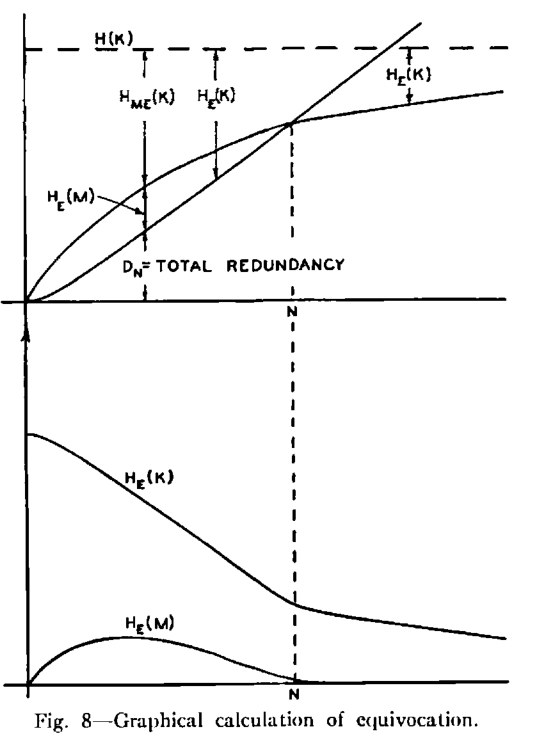
\includegraphics[width=0.8\textwidth]{fig8.png}
	\caption{疑义度的图形化计算}
	\label{fig:fig8}
\end{figure}

\begin{figure}[htbp]
	\centering
	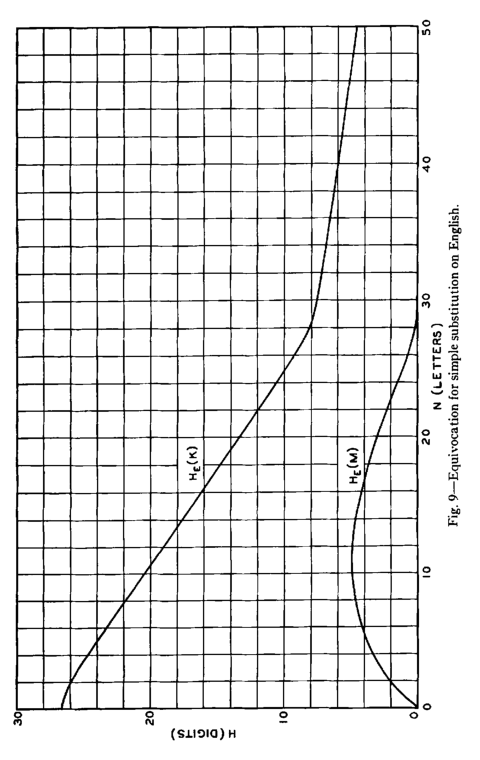
\includegraphics[width=0.8\textwidth]{fig9.png}
	\caption{英文的简单替换疑义度}
	\label{fig:fig9}
\end{figure}

对于周期d(随机密钥)的换位(tranposition),$H(K)=\log{d!}$,或大约$d\log{d/e}$(使用d!的斯特林近似)。如果我们将每个字母的0.6(十进制数)作为适当的冗余,记住字母频次的保留,我们将获得大约$1.7d\log{d/e}$作为唯一解距离。这在实验上也很好地验证了。注意,在这种情况下,$H_E(M)$仅定义为d的整数倍。

对于维吉尼亚,唯一解点将出现在大约2d个字母处,这也是正确的。具有与简单替换相同密钥大小的维吉尼亚特性近似如图10所示,与简单的替换和换位相比,Playfair和Fractional情况更可能遵循随机密码的理论公式。这是因为它们更复杂,并为它们操作的消息提供更好的混合特性。

\begin{figure}[htbp]
	\centering
	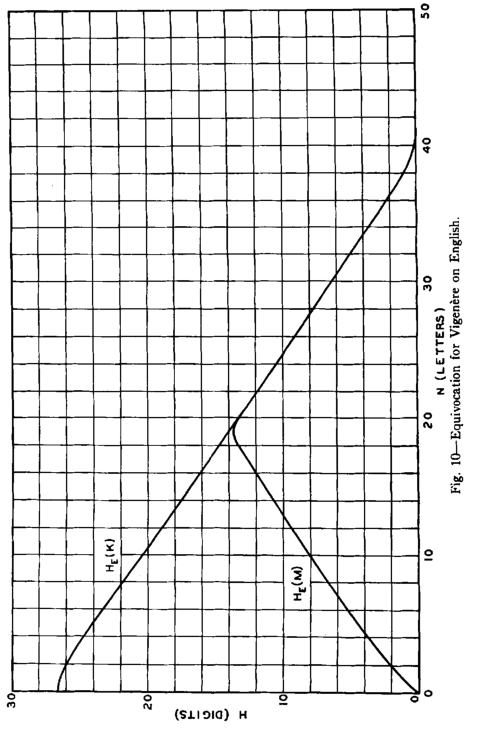
\includegraphics[width=0.8\textwidth]{fig10.png}
	\caption{英文的维吉尼密码的疑义度}
	\label{fig:fig10}
\end{figure}

混合字母维吉尼亚(d个字母中的每一个独立混合并按顺序使用)密钥空间大小为:
\[H(K)=d\log{26!}=26.3d\]
,其唯一性点应为大约53d个字母。

这些结论也可以用凯撒型密码进行粗略的实验测试。在第11节的表I中分析的特定密码中,函数($H_E(K,N)$)已被计算并与随机密码的值一起在下面给出。\par
\vspace{0.5cm}
\begin{minipage}{\textwidth}
	\centering
	%\begin{table}		
		\begin{tabular}{c|c|c|c|c|c|c}
			\hline 
			N& 0 & 1 & 2 & 3 & 4 & 5 \\ 
			\hline 
			H(observed)& 1.41 & 1.24 & .97 & .60 & .28 & 0 \\ 
			\hline 
			H(calculated)& 1.41 & 1.25 & .98 & .54 & .15 & .03 \\ 
			\hline 
		\end{tabular} 
	%\end{table}
\end{minipage}
\par
\vspace{0.5cm}
一致性被认为是非常好的,尤其是我们要意识到,观察到的H实际上是许多不同密码的平均值,并且N较大时,D只是粗略估计的。

由此看来,随机密码分析可以用于估计普通类型密码的疑义度特征和唯一解距离。

\newpage
%---------------------------------------------
%   
%     16.VALIDITY OF A CRYPTOGRAM SOLUTION
%
%---------------------------------------------

\section{密文方案的有效性(VALIDITY OF A CRYPTOGRAM SOLUTION)}

有时疑义度公式与密码工作中出现的问题有关,这些问题涉及到所谓的密文破解方案的有效性。在密码学的历史上,有许多密码或可能的密码,聪明的分析家已经找到了“解决方案”。然而,它涉及到一个复杂的过程,或者材料太少,以至于出现了一个问题,即密码分析家是否在密文中“读到了解决方法”。例如,参见培根莎士比亚密码和“罗杰·培根”手稿。\footnote{ See Fletcher Pratt,loc. cit.}

一般来说,我们可以说,如果所提出的系统和密钥方案,破解所需截取材料长度远大于唯一解距离,则此加密方案是可信的。如果材料与唯一解距离级数相同或短于唯一性距离,则此加密方案不太可信。

可以用另一种有用的方式来考虑冗余在逐渐确定密文的唯一解方案中的作用。冗余本质上是消息字母上的一系列条件,确保其在统计上是合理的。这些一致性条件在密文中产生相应的一致性条件。密钥赋予密文一定的自由度,但随着越来越多的字母被拦截,一致性条件耗尽了密钥所允许的自由度。
最终,只有一个消息和密钥满足所有条件,我们有了唯一解方案。在随机密码中,一致性条件在某种意义上与“密钥颗粒”“正交”,在尽可能快地消除消息和密钥方面具有效果。
这是通常情况。然而,通过适当的设计,可以将语言的冗余与“密钥颗粒”“对齐”,从而自动满足一致性条件,并且$H_E(K)$不接近零。这些“理想”系统,将在下一节中讨论,具有这样一种性质,即变换$T_i$都在E空间中产生相同的概率。


\newpage
%---------------------------------------------
%   
%     17.IDEAL SECRECY SYSTEMS
%
%---------------------------------------------

\section{理想保密系统(IDEAL SECRECY SYSTEMS)}

我们已经看到,如果我们允许消息是无限长的,那么完全保密需要无穷数量的密钥。密钥可选范围有限时,密钥和消息的疑义度通常会接近0,但也不是必然这样。事实上,$H_E(K)$有可能保持在初始值常数$H(K)$上,那么无论截获多少材料,依然没有一个唯一的解决方案,除了得到很多可以相互比较的概率。我们把理想系统(ideal system)定义为:当$N\rightarrow \infty$时,$H_E(K)$和$H_E(M)$不趋近0的系统。我们把“强理想系统”(strongly ideal)定义为:$H_E(K)$保持在常数$H(K)$的系统。

一个例子是一种人工语言的简单替换,其中所有字母都是等概率的,连续的字母是独立选择的。很容易看出,$H_E(K)=H(K)$和$H_E(M)$沿着斜率$\log{G}$(其中G是字母表中的字母数)直线上升,直到到达$H(K)$,之后保持恒定。

在自然语言中,通常可以近似理想的特征————可以使唯一解点出现在所期望的足够大的N上。然而,当我们试图做到这一点时,所需系统的复杂性通常会迅速上升。对于任何有限复杂度的系统,并不总是能够达到理想的特性。

为了近似理想的疑义度,可以首先用一个消除所有冗余的转换器对消息进行处理。在这之后,几乎任何简单的加密系统————置换、换位、维吉尼等,都是令人满意的。转换器越精细,输出越接近理想形式,保密系统就越接近理想特性。

\begin{theorem}
	T是强理想的一个充要条件是,对于任意两个密钥,$T_i^{-1}T_j$是在消息空间本身的保测变换。
\end{theorem}

确实是这样,因为当且仅当满足该条件时,每个密钥的后验概率等于其先验概率。\par

\vspace{1cm}
************************************************\par
\textbf{译者注:}\par
在数学中,某个集合$X$上的$\delta$代数($\delta$-algebra)又叫$\delta$域,是X的所有子集的集合(也就是幂集)的一个子集。这个子集满足:对于可数个集合的并集运算和补集运算的封闭性(因此对于交集运算也是封闭的)。$\delta$代数可以用来严格地定义所谓的“可测集”,是测度论的基础概念之一。\par

\begin{definition}[$\delta$代数]
	设
	$r$是由集合$X$中一些子集所构成的集合族(也叫做集类),且满足下述条件:
	\begin{itemize}
		\item $X\in r$;
		\item 若$A\in r$,则$A$的补集$A^c \in r$;
		\item 若$A_n\in r$,$n=1,2,\ldots$,则$\cup A_n \in r$;
	\end{itemize}
	我们称$r$是一个$\delta$代数。
\end{definition}

数学上,测度(Measure)是一个函数,它对一个给定集合的某些子集指定一个数,这个数可以比作大小、体积、概率等等。传统的积分是在区间上进行的,后来人们希望把积分推广到任意的集合上,就发展出测度的概念,它在数学分析和概率论有重要的地位。\par

\begin{definition}[测度]{}
	$r$是集合$X$上的一个$\delta$代数,$X$的一个测度是一个函数$\mu : r\longmapsto [0,+\infty]$,且满足下述条件:
	\begin{itemize}
		\item 非负性(Non-negativity): 对任何子集$A\in r$, $\mu (A) \geq 0$;
		\item 非空集合(Null empty set): $\mu(\phi) = 0$,$\phi$表示空集;
		\item 可数加(Countable additivity): 对任何可数序列$(A_1,A_2,A_3,\ldots)$,两两不想交,$A_i\cap A_j=\phi (i\neq j)$,我们有
		$\mu (\cup_{i=1}^{\infty} A_i)= \sum_{i=1}^{\infty} \mu(A_i)$ ;
	\end{itemize}
\end{definition}

\begin{definition}[测度空间]
	设$X$为集合,$r$为$X$的子集组成的$\delta$代数,$\mu$为$r$上的非负测度,则三元组$(X,r,\mu)$称为测度空间。
\end{definition}

\begin{definition}[概率空间]
	设$X$是非空集合,也称“样本空间”,$r$是$\delta$代数,$P$为$r$上的非负测度,$(X,r,P)$称为测度空间,如果总测度为1,即$P(X)=1$,称此测度空间为概率空间。
\end{definition}

\begin{definition}[可测影射]
	设$(X,r,P)$为概率空间,对于任何$A\in r$,有
	\[T^{-1}A=\{\omega:T\omega \in A\} \in r\]
	则空间$r$到自身的影射$T$称做可测的。
\end{definition}

\begin{definition}[保测变换(measure-preserving transformation)]
	设$(X,r,P)$为概率空间,如果对于任何$A\in r$,有
	\[P(T^{-1}A)=P(A)\]
	则可测影射$T$称做保测变换。
\end{definition}
************************************************\par
\vspace{1cm}
\newpage
%---------------------------------------------
%   
%     18.EXAMPLES OF IDEAL SECRECY SYSTEMS
%
%---------------------------------------------

\section{理想保密系统的例子(EXAMPLES OF IDEAL SECRECY SYSTEMS)}

假设我们的语言由一系列字母组成,这些字母都是以相等的概率独立选择的。然后冗余度为零,根据第12节的结果,$H_E(K)=H(K)$。我们得到以下结果。

\begin{theorem}
	如果所有字母的可能性相等且独立,则任何闭合密码(closed cihper)都是强理想的。
\end{theorem}

消息的疑义度将沿着密钥表现特征(appearance characteristic)上升,通常会接近$H(K)$,尽管在某些情况下不会。
在n-字母替换、换位、维吉尼亚及其变种、分馏等情况下,这种简单语言是强理想系统,所以当$N\rightarrow \infty,H_E(M)\rightarrow H(K)$。

理想保密系统有以下几个缺点:
\begin{enumerate}
	\item 系统必须与语言紧密匹配。这需要设计者对语言的结构进行深入地研究。此外,统计结构的变化或从可能的消息集合中进行选择,如在可能的单词(该特定密文中预期的单词)的情况下,会使系统容易分析。
	\item 自然语言的结构极其复杂,这意味着消除冗余需要复杂的转换。因此,必须考虑执行这一操作的机器,至少在信息存储方面要考虑,因为预期会需要一部比普通字典更大的“字典”。
	\item 一般来说,所需的转换会引入错误特征的不良传播。单个字母传输中的错误会在其附近产生一个变化区域,其大小与原始语言中统计效应的长度相当.
\end{enumerate}

\newpage
%---------------------------------------------
%   
%     19.FURTHER REMARKS ON EQUIVOCATION AND REDUNDANCY
%
%---------------------------------------------

\section{关于疑义度和冗余的进一步评论(FURTHER REMARKS ON EQUIVOCATION AND REDUNDANCY)}

我们将“普通英语”的冗余度取为每个字母大约0.7或50\%的冗余度。这是基于省略了单词划分的假设。这是一个基于统计结构的近似数字,延伸了大约8个字母,并假设文本为普通类型,如报纸写作、文学作品等,这里我们记录了一种粗略估计这个数字的方法,这是密码学感兴趣的。

运行密钥密码是一种Vernam类型的系统,其中,密钥不是随机字母序列,而是一个有意义的文本。现在已知,运行密钥密码通常可以唯一地求解。这表明英语可以减少二分之一,这意味着至少有50\%的冗余。然而,由于一些原因,这个数字不能增加太多,除非考虑英语的长范围“意义”结构。

运行密钥密码可以很容易地改进,从而得到没有密钥就无法求解的密码系统。如果一个人用大约4个不同的文本作为密钥,来加密一个英文文本,并把它们都添加到消息中,那么就有足够的密钥被引入,从而产生高的正向疑义度。
另一种方法是使用文本的每第10个字母作为密钥,中间的字母省略,省略的不能在消息的任何其他点使用。这有很多相同的效果,因为这些间隔字母几乎是独立的。

一段文字中的元音可以被省略而不会有本质的损失,这一事实表明了一种可以大大改进几乎所有密码系统的简单方法。
首先删除所有元音,或尽可能多地删除信息,而不存在多次重构的风险,然后对剩余部分进行加密。
因为这样可以将冗余度降低$\frac{1}{3}$或$\frac{1}{4}$,所以唯一解点将被这个因子移出。这是接近理想系统的一种方法——将解码者(decipher)的英语知识作为解码系统的一部分\footnote{译者注:这句话原文是“”using the decipher's knowledge of English as part of the deciphering system",此处decipher没有翻译为“破解者”,因为破解者一定会将其各种知识用于破解,译者认为这里的意思应该是:在设计解码系统时,考虑到我们对于英文的知识,并且将这个考虑应用到解码中,这种考虑是去除些知识对破解的指导,这使得破解更加困难。}。


\newpage
%---------------------------------------------
%   
%     20.DISTRIBUTION OF EQUIVOCATION
%
%---------------------------------------------

\section{疑义度分布(DISTRIBUTION OF EQUIVOCATION)}

疑义度的分布可以为应用于语言的保密系统,提供比疑义度特征更完整的描述。对于截获的N个字母,我们考虑疑义度(对于这些特定的E,而不是$H_E(M)$的平均值)位于特定区间的密文片段。这给出了N个字母的H位于H和H+dH之间的概率密度分布函数:
\[P(H_E(M),N) dH_E(M)\]
我们之前研究的平均疑义度就是这种分布的平均值。
函数$P(H_E(M),N)$可以被认为是$H_E(M)$在N平面上沿着垂直于纸张的第三维度绘制的。如果语言是纯的,影响范围很小,并且密码是纯的,那么函数通常是这个平面中的一个脊,其最高点近似于平均值$H_E(M)$,至少接近唯一解点。在这种情况下,或者当条件几乎得到验证时,平均曲线给出了系统的合理完整的图。

另一方面,如果语言不是纯的,而是由以下一组纯组件组成的,
\[L=\sum {p_i L_i}\]
它们与系统具有不同的疑义度曲线,那么总分布通常由一系列脊组成。
根据其$p_i$加权的每个$L_i$,平均疑义度特性将是这些山脊中间的一条线,可能无法给出非常完整的情况图,如图11所示。如果系统不是纯的,而是由几个具有不同H曲线的系统组成,则会出现类似的效果。

\begin{figure}[htbp]
	\centering
	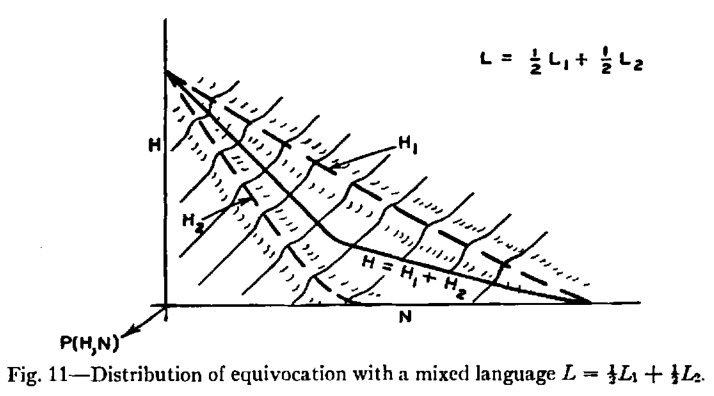
\includegraphics[width=0.8\textwidth]{fig11.png}
	\caption{混合语言$L=\frac{1}{2}L_1 + \frac{1}{2}L_2$的疑义度分布}
	\label{fig:fig11}
\end{figure}

混合统计结构上彼此接近的纯语言的效果是增加脊的宽度。
在唯一解点附近,这往往会提高疑义度的平均值,因为疑义度不能变为负的,而扩散主要是正的方向。因此,我们预计,在这个区域,基于随机密码的计算量应该是比较低的。

\newpage
%---------------------------------------------
%   
%     21.THE WORK CHARACTERISTIC
%
%---------------------------------------------

\begin{center}
	%\section*
	\LARGE{\textbf{第三部分\ 实际保密(PRACTICAL SECRECY)}}
\end{center}

\section{工作特性(THE WORK CHARACTERISTIC)}

在拦截的材料经过唯一解点后,通常会有密码的唯一解。将这种高概率的唯一解分离出来的问题就是密码分析的问题。在唯一解点之前的区域,我们可以说密码分析的问题是隔离所有高概率的可能解(与其余的解相比),并确定它们的各种概率。

虽然原则上总是可以确定这些解决方案(例如,通过对每个可能的密钥进行试验),但不同的加密系统在破解所需工作量方面表现出很大的差异。确定一个由N个字母组成的密文$W(N)$的密钥的平均工作量,以人时度量,可以称为系统的工作特性。
这个平均值是所有消息和所有密钥对应概率确定。函数$W(N)$是系统提供的“实际保密”量的衡量标准。

对于一个简单的英语替代,其工作和疑义度特征如图\ref{fig:fig12}所示。
曲线的虚线部分位于有许多可能解的范围内,这些解都必须被确定。在唯一解点之后的固定部分中,一般只存在一个解,但如果只给出很少的必要数据,则必须做大量的工作来分离它。随着可用材料的增加,工作量迅速减少到某个渐近值,在这个值中,额外的数据不再减少工作量。

\begin{figure}[htbp]
	\centering
	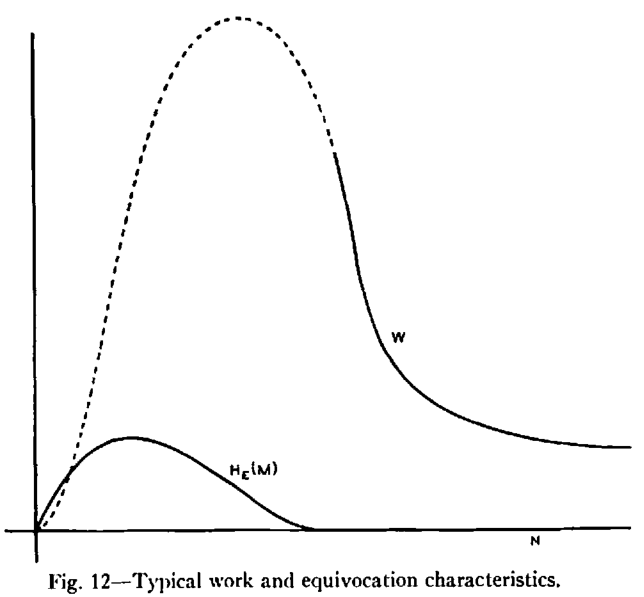
\includegraphics[width=0.8\textwidth]{fig12.png}
	\caption{典型工作和疑义度特征}
	\label{fig:fig12}
\end{figure}

从本质上讲,图\ref{fig:fig12}所示的行为发生在任何类型的保密系统中,其中疑义度接近于零。然而,即使$H_E(M)$曲线大致相同,不同类型的密码所需的工时规模也会有很大差别。
例如,具有相同密钥空间大小的Vigenere或复合Vigenere将具有更好的(即更高的)工作特性。
一个好的实用的保密系统是,它的$W(N)$曲线保持足够高,高到密钥传输的字母数,以防止敌人实际执行解决方案,或者将解决方案延迟到信息被废弃的程度。

我们将在下面几节中考虑保持函数$W(N)$大的方法,即使$H_E(K)$可能实际上为零。这本质上是一个“最大最小”类型的问题,就像我们在智力对抗时经常遇到的情况一样。\footnote{见冯·诺伊曼和摩根斯顿,loc. cil。密码设计师和密码分析师之间的情况可以被认为是一个结构非常简单的“游戏”;这是一个完全信息的零和两人博弈,只有两步棋。密码设计师为他的“移动”选择一个系统。然后密码分析人员被告知这一选择,并选择一种分析方法。游戏的“值”是用所选方法破解系统中密码所需的平均工作量。}
\textbf{在设计一个好的密码时,我们必须最大化敌人破解密码所做工作的最小值。仅仅确保密码分析的标准方法都不起作用是不够的————我们必须确保任何方法都不会轻易破解系统。}\footnote{译者注:这其实是计算复杂度的概念,算法计算复杂度是大约是在$1960\sim 1970$年之间提出并发展起来的,所以香农在写这篇文章是没有算法复杂度这样的理论支撑,但是其在这里提的一些构想或者想法或者思想其实就是密码学计算复杂性定义的思想。}
事实上,这一直是许多系统的弱点;它们被设计用来抵抗所有已知的求解方法,后来又产生了新的密码分析技术,使它们容易被分析。

好的密码设计问题本质上是在一定条件下发现困难的问题。这是一个相当不寻常的情况,因为人们通常是在寻找一个领域中简单和容易解决的问题。

我们怎么能确定一个对于足够大的N有唯一解的系统,需要大量的工作来打破每一种分析方法呢?有两种方法可以解决这个问题;(1)我们可以研究密码分析人员可用的解决方案的可能方法,并试图用足够通用的术语描述它们,以涵盖他可能使用的任何方法。然后我们构造我们的系统来抵抗这种“一般的”解法。(2)我们可以用这样一种方式构造密码:破译它相当于(或需要在过程中的某个时刻)解决已知的费力的问题。因此,如果我们能够证明解一个特定的系统所需要的工作量至少与解一个具有大量未知数的联立方程组所需要的工作量相等,那么我们就可以得到工作特性的一个下界。

接下来的三节将针对这些一般性问题。很难足够精确的定义所涉及的相关思想,并获得数学定理形式的结果,但人们相信,以一般原理形式得出的结论也是正确的。

\newpage
%---------------------------------------------
%   
%     22.THE WORK CHARACTERISTIC
%
%---------------------------------------------

\section{密文解的一般性讨论(GENERALITIES ON THE SOLUTION OF CRYPTOGRAMS)}

在被截获的材料中超过了唯一解距离之后,理论上任何系统都可以通过尝试每一个可能的密钥来求解,直到获得唯一解————也就是说,在原始语言中“有意义”的解密信息。一个简单的计算表明,这种求解方法(我们可以称之为完全试错)是完全不切实际的,除非是在密钥空间小得离谱的情况下。

例如,假设我们有26!个可能的密钥或约26.3位十进制数字,大小与英语的简单替换相同。无论如何,这都是一个小的密钥空间,它可以写在一张小纸条上,也可以在几分钟内记住。它可以存储在27个开关量上,每个开关有10个位置,或者在88个双位置开关。\footnote{译者注:
26!种可能的密钥,密钥的熵为$-\sum_{1}^{26!}{\dfrac{1}{26!}\log_{10}{\dfrac{1}{26!}}}=\log_10{26!}\approx 26.6$,这个意思就是用十进制数表示,需要26.6位,这个数字与原文计算的稍有差别。同理用二进制表示需要的位数为$\log_2{26!}=\log_{10}{26!}\div \log_{10}{2}\approx 88.4$,如果每一位用开关记录状态,就需要89个双置开关,这个与原文也有点差别。
}

再进一步假设,为了使密码分析人员获得所有可能的优势,他构建了一个电子设备,以每微秒一个密钥的速度尝试密钥(可能通过$\chi^2$检验从统计显著性的结果中自动选择)。他可能期望在中途找到正确的密钥,经过大约$2\times 10^{26}/2\times 60^2\times 24\times 365\times 10^6$或$3\times 10^{12}$年的时间。\footnote{译者注:这里是将所需微妙换算成年的过程,首先分子是$2\times 10^{26}$,这个采用近似,也就是$26!\approx 2\times 10^{26}$,分母的$10^6$是将微秒换算为秒,分母的$60^2$是将秒换算成小时,分母的24是将小时换算为天,365是将天换算为年,分母的2,是因为假设中途就找到密钥,也就是只试了一半密钥。}

换句话说,即使是一个很小密钥空间,完全的试错也永远不会被用于破解密文,除非在密钥非常小的情况下,例如只有26种可能性或1.4位数字的Caesar密码\footnote{译者注:1.4是指的密钥的信息量,每个密钥的可能性相同,$\log_{10}{26}\approx 1.4$}。在密码学中经常使用的试错法是另一种方法,或者通过其他方法加以加强。如果一个人有一个秘密系统,需要完全的试错,它将是极其安全的。如果有意义的原始信息,比如1000个字母,是从1000个字母的所有序列中随机选择出来的,就会产生这样一个系统。任何一种简单的密码被应用到这种语言中,那就不可能有比完全试错改进多少的方法。

实际使用的密码分析方法通常涉及大量的试错,但方法不同。首先,试验从可能性较大的假设发展到可能性较小的假设;其次,每次试验都要处理一大组密钥,而不是单一的一个。因此,可以将密钥空间划分为10个子集,每个子集包含大约相同数量的密钥。最多10次试验就能确定哪个子集是正确的。然后将这个子集划分为几个次要子集并重复此过程。在相同的密钥空间大小($26!\approx 2\times 10^{26}$)下,通过完全的试错,我们预计大约$26\times 5$或130次试验,而不是$10^{26}$次。
首先选择子集中可能性最大的进行检验,这将进一步提高速度。
如果将试验分为两个部分(这是减少试验次数的最佳方法),则只需要88次试验。\footnote{译者注:需要88次实验可以这样计算,第一次分$\dfrac{26!}{2}$,第二次分$\dfrac{26!}{2^2}$,第三次分$\dfrac{26!}{2^3},\ldots$,可见2的幂次就是分的次数,那么总共分的次数就是$\log_2{26!}\approx 88$}完全试错需要按密钥数的顺序进行试错,而这种细分试错的次数是密钥位数,只需要按顺序进行试错。

即使不同的密钥有不同的概率,这也是正确的。因此,要使试验的预期次数最小化,正确的方法是将密钥空间划分为等概率的子集。当确定了恰当子集时,再将其细分为等概率子集。如果这一过程可以继续,那么当每个划分为两个子集时,预期的试验数量将为
\[h=\dfrac{H(K)}{\log{2}}\]

如果每个测试有S个可能的结果,并且每个结果都对应于密钥位于S个等概率子集中的一个,则预期测试数为:
\[h=\dfrac{H(K)}{\log{S}}\]
应注意这些结果的直观意义。在具有等概率性的两室测试(two-compartment test )中,每个测试都会产生一位关于密钥的信息。如果子集具有非常不同的概率,如在完全试错中测试单个密钥,则只能从测试中获得少量信息。
因此,26!个等概率密钥,一个测试只产生
\[-\left[\dfrac{26!-1}{26!} \log{\dfrac{26!-1}{26!}}+\dfrac{1}{26!}\log{\dfrac{1}{26!}}\right]\]
或大约$10^{-25}$比特的信息。分成S个等概率子集使每次试验获得的信息达到最大值$\log{S}$,而预期的试验次数是要获得的总信息,即$H(K)$,除以这个量。

这里的问题类似于最近流传的各种硬币称重问题。一个典型的例子如下:已知,27枚硬币中有一枚是假的,而且比其他硬币稍轻。有了化学家的天平,假币就可以通过一系列的称重来分离出来。做这件事所需的最小称重次数是多少?正确答案是3,首先将硬币分成三组,每组9个。其中的两个在天平上比较。三个比较结果决定了包含赝品的集合,这个集合再被分成3个子集,每个子集3个,然后继续这个过程。一组硬币对应一组密钥,假硬币对应正确的钥匙,称重过程对应一个试验或测试。初始不确定度为$\log_2{27}$bits,每次试验产生$\log_2{3}$位的信息;因此,当没有“丢番图麻烦(diophantine trouble)”时,$\log_2{27}/\log_2{3}$或3次试验就足够了。

这种求解方法只有在密钥空间可以被划分为少数子集的情况下才可行,并且有一个确定正确密钥所属子集的简单方法。为了应用一致性测试并确定假设是否成立,不需要假设密钥完全准确,只需要对密钥某部分(或密钥是否在密钥空间的某个大片段中)的假设进行测试。换句话说,可以分位解密并逐位地确定密钥。

这种分析方法的可能性是大多数密码系统的关键弱点。例如,在简单替换中,对单个字母的假设可以根据其频率、通信的种类、重复或反转等进行检查。在确定单个字母时,密钥空间从原来的26减少了1.4。在所有基本类型的密码中都可以看到同样的效果。在维吉尼亚密码中,通过破译这个片段的其他点,并注意是否明文出现,可以很容易地验证密钥的两到三个字母的假设。从这个角度来看,复合维吉尼亚密码要好得多,如果我们假设有相当多的合成周期,产生的重复率大于将被拦截的重复率。在这种情况下,加密每个字母时使用的密钥字母和周期的数量一样多。尽管这只是整个密钥的一小部分,但在应用一致性检查之前,至少必须假设有相当数量的字母。

关于实际的小密钥密码设计,我们的第一个结论是,应该使用相当数量的密钥对消息的每个小元素进行加密。

\newpage
%---------------------------------------------
%   
%     23.STATISTICAL METHODS
%
%---------------------------------------------

\section{统计方法(STATISTICAL METHODS)}

通过统计分析可以解决多种密码,我们依然以简单替换为例。密码分析师对截获的密码所做的第一件事是进行频率计数。如果密文包含,比方说,200个字母,那么可以安全地假设只有很少(如果有的话)字母超出频率组的范围,将统计的频次划分为4组具有明确定义评率限制的集合。在此限值内的密钥数的对数可以计算为
\[\log{2!9!9!6!}=14.28\]
,简单的频次计数因此将密钥的不确定性减少了12位小数,这个减少的量很大。\footnote{译者注:在没有频次统计情况下,密钥的信息量为$\log_{10}{26!}\approx 26.6$,大约是26位十进制,进行频次统计后变为14.28,所以此处说减少了12位。}

一般来说,统计攻击的过程如下:在截获的密文E上测量某个统计值。这个统计是这样的,对于所有合理的消息M,它假设有大约相同的值$S_K$,该值仅取决于所使用的特定密钥K。
由此获得的值用于将可能的密钥限制为那些将在所观察到的值的邻域中给出S值的密钥。
这样得到的值将可能的密钥限制为可以获得观察值附件的S值,一个不依赖于K的统计量,或者一个随M和随K变化一样多的统计量,在限制K方面没有价值。因此,在换位密码中,字母的频率计数不能给出关于K的信息——每一个K都使这个统计量保持不变。因此,在破译换位密码时不能使用频率计数。

更准确地说,我们可以将“解决能力”归因于给定的统计数据S。对于S的每一个值都有一个密钥$H_S(K)$的条件疑义度,当给定S值时,正如我们所知道的,疑义度与密钥相关。这些值的加权平均\[\sum{P(S)H_S(K)}\]此式给出了当S已知时,密钥的平均疑义度,其中,$P(S)$是S为特定值时的先验概率,密钥大小$H(K)$(小于平均疑义度)衡量统计量S的“求解能力”。

在强理想密码中,密码的所有统计量都与所使用的特定密钥无关。这就是$T_jT_k^{-1}$在E空间上或$T_j^{-1}T_k$在M空间上的保测度性质(measure preserving property)。

统计数据有好有坏,就像试错方法有好有坏一样。事实上,一个假设的试错测试是一种统计,上面所说的关于最佳试验类型的说法是普遍成立的。解一个系统的一个好的统计量必须具有以下性质:
\begin{enumerate}
	\item 它必须是容易测量的。
	\item 如果要求求解密钥,这个统计量必须更多地依赖于密钥而不是消息,M的变化不应该掩盖它与K的变化。 
	\item 尽管M的变化产生了“模糊性”,但可以“解析”的统计值应该将密钥空间划分为若干具有可比概率的子集,统计值指定正确密钥所在的那个子集。统计数据应该为我们提供关于密钥的大量信息,而不是一小部分。
	\item 它提供的信息必须是简单和可用的。因此,定位密钥所在子集的统计信息必须是密钥空间的一个简单属性(nature)。
\end{enumerate}

简单替换的频率计数是一个非常好的统计的例子。

\textbf{有两种方法(除了求助于理想系统)会使统计分析受挫。我们可以把这些方法称为扩散法(diffusion)和混淆法(confusion)}。在扩散方法中,导致其冗余的M的统计结构被“消散”为长程统计,即,成为包含密文中字母长组合的统计结构。这里的效果是,敌人必须拦截大量的材料来绑住这个结构,因为该结构只有在非常小的单个概率的块中才明显。此外,即使他有足够的资料,所需要的分析工作也要大得多,因为冗余分散在大量的个别统计数据上。统计量扩散的一个例子是使用“平均”操作对消息$M=m_1,m_2,m_3,\dots$进行操作,如
\[y_n=\sum_{i=1}^{s} m_{n+i}\mod{26}\]
将消息的s个连续字母相加,得到字母$y_n$,可以证明,$y$序列的冗余度与$m$序列的冗余度相同,但结构已经消散。因此,$y$中的字母频率将比$m$中的字母频率更接近相等,双字母频率也更接近相等,等等。事实上,任何可逆操作,只要输出一个字母,输入一个字母,并且没有无限的“内存”,就会有一个与输入相同的冗余输出。如果不进行压缩,统计数据永远无法消除,但它们可以扩散。


混淆法是E的简单统计量和K的简单描述之间的关系变成非常复杂。在简单替换的情况下,很容易描述字母频次E对于K的限制。如果连接非常复杂和混乱,敌人可能仍然能够评估统计数据$S_1$,这将把密钥限制在密钥空间的某个区域。然而,这个限制是空间中的某个复杂区域R,可能“折叠”了很多次,敌人很难利用它。第二个统计量$S_2$将K进一步限制在$R_2$,因此它位于相交区域;但这并没有太大的帮助,因为很难确定交集是什么。

更准确地说,让我们假设密钥空间有他希望确定的“自然坐标”$k_1,k_2,\ldots,k_p$。比方说,他测量一组统计数据$s_1,s_2,\ldots,s_n$,这些足以确定$k_i$。然而,在混淆法中,连接这些变量集的方程是复杂的。我们有:
\[f_1(k_1,k_2,\ldots,k_p)=s_1\]
\[f_2(k_1,k_2,\ldots,k_p)=s_2\]
\[\ldots\]
\[f_n(k_1,k_2,\ldots,k_p)=s_n\]
所有的$f_i$涉及所有的$k_i$,密码学家必须同时解决这个系统 ———— 这是一项困难的工作。在简单的(不是混淆的)情况下,函数只涉及到$k_i$的一小部分 ———— 或者至少其中一些是,那么可以首先解决简单的方程,计算$k_i$中的一些值,然后把它们代入更复杂的方程中。

这里的结论是,对于一个好的加密系统,应该采取步骤进行冗余的扩散或混淆(diffuse or confuse)(或两者兼具)。


\newpage
%---------------------------------------------
%   
%     24.THE PROBABLE WORD METHOD
%
%---------------------------------------------


\section{可能词方法(THE PROBABLE WORD METHOD)}


破解密码最有力的工具之一是使用可能的词。可能出现的单词是来源在特定信息中出现的单词或短语,也可能是在该语言的任何文本中出现的常见单词或音节,如英语中的The、and、lion、that等。

一般来说,可能词方法是这样使用的:假设一个可能的词在明文的某个地方,那么密钥或部分密钥就确定了。这用于破译密码的其他部分,并提供一致性测试。如果其他部分是明文,假设是合理的。

经典密码中很少有使用小密钥并能抵抗长时间的概率字分析的。从这种方法的考虑,我们可以建立一个可以被称为酸性测试的密码测试。它只适用于密钥很小的密码(少于50位十进制数字)\footnote{译者注:50位十进制数,最大为50个9,十六进制表示为“446c3b15f9926687d2c40534fdb563ffffffffffff”,共42个十六进制位,如果用二进制表示为“ 1000100011011000011101100010101111110011001001001100110
	10000111110100101100010000000101001101001111110110110101011000111111111
	11111111111111111111111111111111111111111 ”,共167比特。},适用于自然语言,并且不使用理想的方法获得机密性。酸性测试是:知道一小部分信息和对应的密文,确定密钥或密钥的一部分有多难?在任何容易做到这一点的系统中,都不可能有很强的抵抗力,因为密码分析师总是可以利用可能的词,结合试错,直到得到一致的解决方案。


(限制)密钥大小的条件使试错的数量减少,关于理想系统的条件是必要的,因为这些条件会自动给出一致性检查。自然语言的假设暗示了可能词和短语的存在。

请注意,在这些条件下的解难求,与加密和解密是简单过程的要求并不矛盾。加密的函数符号:
\[E=f(K,M)\]
解密是:
\[M=g(K,E).\]

这两个都是对参数的简单运算,第三个方程
\[K=h(M,E)\]
就不容易计算了。

我们还可以指出,在研究一种新型密码系统时,最好的攻击方法之一是考虑如果给定足够的M和E,如何确定密钥。

混淆原理可以(而且必须)用于给使用可能词技术的密码分析人员制造困难。给定(或假设)$M=m_1,m_2,\ldots,m_s$和$E=e_1,e_2,\ldots,e_s$,密码分析师可以为不同的密钥元素$k1,k2,\ldots,kr$建立方程(即加密方程)。
\[e_1=f_1(m_1,m_2,\ldots,m_s;k_1,\ldots,k_r)\]
\[e_2=f_2(m_1,m_2,\ldots,m_s;k_1,\ldots,k_r)\]
\[\ldots\]
\[e_s=f_s(m_1,m_2,\ldots,m_s;k_1,\ldots,k_r)\]

我们认为一切都是已知的,除了$k_i$。因此,每个方程在$k_i$方面都应该是复杂的,并且涉及到许多$k_i$。否则敌人可以先解决简单的问题,再通过代入解决更复杂的问题。

从增加混乱的角度来看,最好是让$f_i$包含几个$m_i$,特别是如果这些$m_i$不相邻,因此相关性较低。然而,这引入了错误传播的不良特性,因为在解码过程中,每个$e_i$通常会影响几个$m_i$,一个错误会传播到所有这些解密的消息中。

为了保持较高的工作特性,在从消息中获取任何密文字母时,密钥的大部分应参与使用。此外,如果可以容忍一些误差传播,则可以进一步依赖几个不相关的$m_i$。我们在这些章节的三个论点的指导下考虑“混合变换”。

\newpage
%---------------------------------------------
%   
%     25.MIXING TRANSFORMATIONS
%
%---------------------------------------------


\section{混合变换(MIXING TRANSFORMATIONS)}

在概率论的某些分支中已经证明有价值的一个概念是混合变换的概念。假设我们有一个概率或者说度量空间$\Omega$和空间到自身的保测变换$F$,也就是说,
一个变换使得变换后的区域FR等于初始区域R的测度。
这个变换叫做混合变换,如果对于空间和区域R上的任意函数,此函数在区域$F^{n}R$上的积分,当$n\rightarrow \infty$时,趋近于函数在整个空间$\Omega$乘以R的积分。
这意味着,如果多次施加F,任何初始区域R都会在整个空间中以均匀的密度混合。通常,$F^{n}R$会变成一个由大量分布在$\Omega$上的细丝组成的区域。随着n的增加,细丝会变得更细,密度也更恒定。

这种精确意义上的混合变换只能发生在具有无穷多个点的空间中,因为在有限点空间中,变换必须是周期性的,简单说,我们可以把混合变换看作是一种将空间中任何合理相联区域均匀分布在整个空间上的变换。\footnote{译者注:目前利用计算复杂度理论设计的密码体系,是否任然满足这一描述?}如果第一个区域可以用简单的术语描述,那么第二个区域将需要非常复杂的术语。

在密码学中,我们可以把所有长度为N的可能消息看作空间$\Omega$,把高概率消息看作区域$R$,后一类的统计结构相当简单。如果应用混合变换,高概率信息将均匀地分散在整个空间。

好的混合变换通常是由两个简单的非交换操作的乘积形成的。Hopf\footnote{E. Hopf,“On Causality , Statistics and Probability,” Journal of Math , and Physics ,v.13,pp.51-102,1934 }已经证明,例如,可以通过这样的操作序列来混合面团,面团首先被擀成薄片,然后折叠,然后卷起,然后再折叠,等等。

在具有自然坐标$X_1,X_2,\ldots,X_s$的空间的良好混合变换中,通过将点$X_i$变换为点$X_i^{'}$,
\[X_i^{'}=f_1(X_1,X_2,\ldots,X_s),i=1,2,\ldots,s\]
,函数f很复杂,以“敏感”的方式涉及所有变量。任何一个$X_\delta$\footnote{译者注:原文不太清晰看着像$X_3$,但是译者觉得应该是$X_\delta$。}的微小变化,都会极大地改变所有的$X_i^{'}$。如果$X_\delta$遍历了它可能的变化范围,点$X_i^{'}$走出一个绕空间的长长的弯曲路径。

可以设计各种适用于自然语言的统计序列混合方法。一个看起来相当不错的方法是一个基本换位,然后是一系列替换和简单线性交替操作,例如,mod 26加相邻字母。我们可以采取
\[F=LSLSLT\]
此处T是换位(tansposition),L是线性运算,S是替换(substitution).

\newpage
%---------------------------------------------
%   
%     26.CIPHERS OF THE TYPE $T_k F S_j$
%
%---------------------------------------------

\section{$T_k F S_j$类型密码(CIPHERS OF THE TYPE $T_k F S_j$)}

假设F是一个很好的混合变换,可以应用到字母序列上,$T_k$和$S_j$是任意两个简单的变换族,即两个简单的密码系统,它们也可能是相同的。就具体性而言,我们可以认为它们都是简单的替换。

从TFS的工作特性来看,它将是一种很好的保密系统。首先,在回顾我们关于统计方法的论点时,我们很清楚,任何简单的统计量都不能提供有关密钥的信息 ———— 从E派生的任何重要统计量都必须是高度相关和非常敏感的类型 ———— 冗余已经被混合变换F扩散(diffuse)和混淆(confuse)了。此外,可能的单词会导致包含所有密钥部分的复杂方程组(当混合良好时),这些方程组必须同时求解(解满足所有方程组)。

有趣的是,如果省略了密码T,剩下的系统与S类似,因此不会更强。敌人仅仅是通过对密码应用$F^{-1}$“解混”,就可解决。如果省略了S,剩下的系统在混合良好的情况下比单独的T强得多,但仍然不能与TFS相比。

通过混合变换分离的简单密码的基本原理当然可以扩展。例如,我们可以使用
\[T_kF_1S_jF_2R_i\]
进行两次混合和三次简单加密。我们还可以通过使用相同的密码,甚至相同的密钥以及相同的混合转换来简化。这很可能简化这类系统的机械化。

将密钥的两个(或多个)出现隔开的混合变换就像敌人的一种屏障 ———— 携带一个已知元素很容易越过这个屏障,但不知此元素(秘钥)却不容易越过。

通过提供两组未知数,S的密钥和T的密钥,并通过混合变换F将它们隔开,我们将未知数“纠缠”在一起,这使破解非常困难。

尽管基于这一原则构建的系统极其安全,但它们有一个严重的缺点。如果混合是好的,那么错误的传播是坏的。一个字母的传输错误将影响多个字母的解密。

\newpage
%---------------------------------------------
%   
%     27.INCOMPATIBILITY OF THE CRITERIA FOR GOOD SYSTEMS
%
%---------------------------------------------

\section{好系统标准的不兼容性(INCOMPATIBILITY OF THE CRITERIA FOR GOOD SYSTEMS)}

第5节中给出的良好保密系统的五个标准在应用于具有复杂统计结构的自然语言时似乎存在一定的不兼容性,在自然语言中,必须做出妥协,并且为了特定的应用,评价必须相互平衡。

如果去掉这五个标准中的任何一个,其他四个标准就可以很好地满足,如下面的例子所示:
\begin{enumerate}
	\item  如果我们忽略第一个要求(保密性),任何简单的密码,如简单替换都可以。在完全忽略这个条件的极端情况下,不需要任何密码,明文发送 !
	\item 如果不限制密钥的大小,则可以使用Vernam系统。
	\item 如果不限制操作的复杂性,可以使用各种极其复杂的加密过程。
	\item 如果我们忽略错误传播条件,TFS类型的系统将非常好,尽管有些复杂。
	\item 如果我们允许大量扩展消息,那么很容易设计出各种系统,其中“正确”的消息与许多“不正确”的消息(错误信息)混合在一起。密钥决定了哪一个是正确的。
\end{enumerate}

对于这五个条件的不兼容,可以给出一个非常粗略的论证:条件5,本文所研究的保密体制都在用;也就是说,没有大量使用空值,等等。完美系统和理想系统分别被条件2、条件3和条件4所排除。因此,1所要求的高度保密必须来自高工作特性,而不是高疑义度特性。如果密钥很小,系统简单,并且错误不传播,那么可能词方法通常会相当容易地破解系统,因为我们有一个相当简单的密钥方程组。

这个推理太模糊了,不足以得出结论,但其大意似乎相当合理。也许,如果各种各样的评价能被赋予数量上的意义,就能找到某种涉及它们的交换方程,并给出物理上最兼容的值集。\textbf{最难用数字衡量的两个方面是运算的复杂性和语言统计结构的复杂性}。

\newpage
%---------------------------------------------
%   
%     APPENDIX
%
%---------------------------------------------
\section*{附录(APPENDIX)}

\subsection*{定理\ref{source:theorem3}证明}
选择任何消息$M_1$,通过任何加密操作$T_i$从$M_1$中获得的所有密文组合在一起,记这组密文为$C_1^{'}$。将通过$T_i^{-1}T_jM_1$获得的消息与$M_1$一起记为$C1$。我们会得到相同的$C_1^{'}$,从C1中任取M,因为\footnote{译者注:原文不太清楚,看似$T_1M_1$,译者觉得应该是$T_iM_1$}:
\[T_sT_j^{-1}T_iM_1=T_iM_1\]
同样可以得到$C_1$.

选择一个不在$C_1$中的M(如果存在这样的M),我们用同样的方法构造$C_2$和$C_2^{'}$。继续以这种方式,我们得到具有属性(1)和(2)的剩余类。设$M_1,M_2$在$C_1$,假设
\[M_2=T_1T_2^{-1}M_1.\]

如果$E_1$在$C_1^{'}$中,并且可以通过
\[E_1=T_{\alpha}M_1 =T_{\beta}M_1= \ldots=T_{\eta}M_1, \]
从$M_1$中获得,则
\[E_1=T_{\alpha}T_2^{-1}T_1M_2 = T_{\beta}T_2^{-1}T_1M_2 = \ldots =T_{\lambda}M_2 = T_{\mu}M_2\ldots\]


因此,$C_1$中的每个$M_i$通过相同数量的密钥转换为$E_1$。同样地,$C'_1$中的每个$E_i$都是由$C_1$中的任意M通过相同数量的密钥得到的。由此可知,密钥的数目是密钥总数的除数,因此我们有属性(3)和(4)。

\newpage
%---------------------------------------------
%   
%     译者注附录:Table I的计算
%
%---------------------------------------------

\section*{译者注附录:Table I的计算}\label{app:table1}

“Secret and Urgent”这一本书的电子版,可以从仓库\url{ https://gitee.com/uisu/InfSecClaT}下的“CTofSecSys”中找到,我们看看本文中的Tabel I中的各个数据是如何计算的。\par
“Secret and Urgent”一书中第252页,有一张统计表“TABLE I Frequent of Occurrence of Letters in English”内容见下:\\
\begin{center}
	\begin{tabular}{|c|c|c|c|}
		\hline 
		& 字母 & 1000个单词中出现的次数 & 1000个字母中出现的次数 \\ 
		\hline 
		1.& E & 591 & 131.05 \\ 
		\hline 
		2.& T & 473 & 104.68 \\ 
		\hline 
		3.& A & 368 & 81.51 \\ 
		\hline 
		4.& O & 360 & 79.95 \\ 
		\hline 
		5.& N & 320 & 70.98 \\ 
		\hline 
		6.& R & 308 & 68.32 \\ 
		\hline 
		7.& I & 286 & 63.54 \\ 
		\hline 
		8.& S & 275 & 61.01 \\ 
		\hline 
		9.& H & 237 & 52.59 \\ 
		\hline 
		10.& D & 171 & 37.88 \\ 
		\hline 
		11.& L & 153 & 33.89 \\ 
		\hline 
		12.& F & 132 & 29.24 \\ 
		\hline 
		13.& C & 124 & 27.58 \\ 
		\hline 
		14.& M & 114 & 25.36 \\ 
		\hline 
		15.& U & 111 & 24.59 \\ 
		\hline 
		16.& G & 90 & 19.94 \\ 
		\hline 
		17.& Y & 89 & 19.82 \\ 
		\hline 
		18.& P & 89 & 19.82 \\ 
		\hline 
		19.& W & 68 & 15.39 \\ 
		\hline 
		20.& B & 65 & 14.40 \\ 
		\hline 
		21.& V & 41 & 9.19 \\ 
		\hline 
		22.& K & 19 & 4.20 \\ 
		\hline 
		23.& X & 7 & 1.66 \\ 
		\hline 
		24.& J & 6 & 1.32 \\ 
		\hline 
		25.& Q & 5 & 1.21 \\ 
		\hline 
		26.& Z & 3 & 0.77 \\ 
		\hline 
	\end{tabular} \par
	英语单词的平均长度是每单词4.5个字母。
\end{center}

从上面这张表中,我们可以看到在1000个字母中各个字母出现频次依次为:\\
$P("C")=\frac{27.58}{1000}=0.02758\approx 0.028$\\
$P("D")=\frac{37.88}{1000}=0.03788\approx 0.038$\\
$P("E")=\frac{131.05}{1000}=0.13105\approx 0.131$\\
$P("F")=\frac{29.24}{1000}=0.02924\approx 0.029$\\
$P("G")=\frac{19.94}{1000}=0.01994\approx 0.020$\\
$\ldots$\\
这就是香农计算的N=1的那一列数据。\par
\vspace{1cm}

“Secret and Urgent”一书中第259页的“TABLE VII Occurrence of Pairs of Letters In English”,可以查出双字母千字出现频次,我们依次查表里出现的双字母频次如下:\\
\begin{tabular}{|c|c||c|c||c|c|}
	\hline
	双字母& 频次 & 双字母 & 频次 & 双字母 & 频次 \\ 
	\hline  
	CR& 6 & DS & 5 & ET & 14 \\ 
	\hline 
	FU& 3 & GV & 0 & HW & 1 \\ 
	\hline 
	IX& 2 & JY & 0 & KZ & 0 \\ 
	\hline 
	LA& 21 & MB & 0 & NC & 19 \\ 
	\hline 
	OD& 6 & PE & 13 & QF & 0 \\ 
	\hline 
	RG& 2 & SH & 14 & TI & 45 \\ 
	\hline 
	UJ& 0 & VK & 0 & WL & 0 \\ 
	\hline 
	XM& 0 & YN & 0 & ZO & 0 \\ 
	\hline 
	AP& 8 & BQ & 0 &  &  \\ 
	\hline 
\end{tabular} 
\vspace{0.5cm}
\par
把所有双字母的频次加起来:
\[6+5+14+3+1+2+21+19+6+13+2+14+45+8=159\]
计算各双字母概率:\\
	$P(cr)=\frac{6}{159}\approx 0.0377$ \\
	$P(ds)=\frac{5}{159}\approx 0.0314$ \\
	$P(et)=\frac{14}{159}\approx 0.0881$ \\
    $\ldots$\par
这个计算结果与本文Table I中N=2这一列的计算结果是一致的。
 
\vspace{1cm}
三字母统计表在“Secret and Urgent”一书中第264页的“TABLE XII English Trigrams”,这个表给出的数字是20,000个单词平均出现次数,我们查表可知:\\
cre频次20\qquad lan频次45\qquad mbo频次4\qquad per频次79\\
shu频次1\qquad tiv频次30\qquad wly频次1\\
只有以上可能,我们把概率和进行归一,先计算频次总数:
\[20   +   45   +   4   +   79   +   1   +   30   +   1 =180\]
各三字母概率为:\\
$P("cre")=\frac{20}{180}\approx 0.1111\quad P("lan")=\frac{45}{180}=0.25$\\
$P("mbo")=\frac{4}{180}\approx 0.0222\quad P("per")=\frac{79}{180}\approx 0.4389$\\
$P("shu")=\frac{1}{180}\approx 0.0056\quad P("tiv")=\frac{30}{180}\approx 0.1667$\\
$P("wly")=\frac{1}{180}\approx 0.0056$\par
这个计算结果与本文Table I中N=3这一列的计算结果是一致的。

\vspace{1cm}
四字母的情况,香农给了一个估算公式:
\[p(ijkl)=p(ijk)p_{jk}(l)\]
根据三字母的情况,我们只需考虑以下情况:\\
$P("crea")=P("cre")P_{"re"}("a")$\qquad $P("lanj")=P("lan")P_{"an"}{"j"}$\\
$P("mbok")=P("mbo")P_{"bo"}("k")$\qquad $P("pern")=P("per")P_{"er"}(“n”)$\\
$P("shuq")=P("shu")P_{"hu"}("q")$\qquad $P("tivr")=P("tiv")P_{"iv"}("r")$\\
$P("wlyu")=P("wly")P_{"ly"}("u")$\\
查三字母频次统计表,可知:\\
"rea"频次82\qquad "anj"频次0\qquad "bok"频次0\qquad "ern"频次34\\
"huq"频次0\qquad "ivr"频次0\qquad "lyu"频次0\\
对于“rea”这种情况,$p_{"re"}("a")$是指出现“re”后,再出现“a”的频次,我们接着查三字母统计表,把所有“re”开头的三字母频次查出如下:\\
\begin{tabular}{|c|c||c|c||c|c|}
	\hline 
	三字母&频次 & 三字母 & 频次 & 三字母 & 频次 \\ 
	\hline 
	rea& 82 & reb & 2 & rec & 45 \\ 
	\hline 
	red& 101 & ree & 45 & ref & 20 \\ 
	\hline 
	reg& 19 & reh & 1 & rei & 8 \\ 
	\hline 
	rel& 12 & rem & 20 & ren & 39 \\ 
	\hline 
	reo& 2 & rep & 28 & rer & 8 \\ 
	\hline 
	res& 114 & ret & 13 & rev & 14 \\ 
	\hline 	
\end{tabular} 
\\
上表中频次之和为:573,我们可知$p_{"re"}("a")=\frac{82}{573}\approx 0.143106$。


对于“ern”这种情况,$p_{"er"}("n")$是指出现“er”后,再出现“n”的频次,我们接着查三字母统计表,把所有“er”开头的三字母频次查出如下:\\
\begin{tabular}{|c|c||c|c||c|c|}
	\hline 
	三字母&频次 & 三字母 & 频次 & 三字母 & 频次 \\ 
	\hline 
	era& 45 & ero & 13 & erd & 6 \\ 
	\hline 
	ere& 162 & erf & 7 & erg & 5 \\ 
	\hline 
	erh& 4 & eri & 36 & erk & 2 \\ 
	\hline 
	erl& 3 & erm & 23 & ern & 34 \\ 
	\hline 
	ero& 7 & erp & 3 & err & 16 \\ 
	\hline 
	ers& 124 & ert & 25 & eru & 17 \\ 
	\hline 	
	erv& 2 & ery & 36 &  &  \\ 
	\hline 
\end{tabular} 
\\
上表中频次之和为:570,我们可知$p_{"er"}("n")=\frac{34}{570}\approx 0.059649$。

我们知道"cre"频次为20,那么按照上面公式“crea”频次大致为$20\times p_{"re"}("a")=20\times 0.143106=2.86212$。


我们知道"per"频次为79,那么按照上面公式“pern”频次大致为$79\times p_{"er"}("n")=79\times 0.059649=4.71227$。

归一化,计算:
\[p("crea")=2.86212 \div (2.86212+4.71227)\approx 0.3779\]
\[p("crea")=4.71277 \div (2.86212+4.71227)\approx 0.6221\]

N=4这一列计算出来的值,与香农先生论文中的数值不符,\textbf{译者没有想到是哪里考虑有误}。

\end{document}

